\svnkwsave{$RepoFile: elton/blog/proforma.tex $}
\svnidlong {$HeadURL: svn://zero.physics.gatech.edu/elton/blog/proforma.tex $}
{$LastChangedDate: 2015-04-17 13:52:46 -0400 (Fri, 17 Apr 2015) $}
{$LastChangedRevision: 311 $} {$LastChangedBy: predrag $}
\svnid{$Id: proforma.tex 311 2015-04-17 17:52:46Z predrag $}


\chapter{Cartan magic}
\label{chap:proforma}


\section{Daily blog}
\label{sect:proformaBlog}

\noindent
$\footnotemark\footnotetext{{\tt \svnkw{RepoFile}}, rev. \svnfilerev:
 last edit by \svnFullAuthor{\svnfileauthor},
 \svnfilemonth/\svnfileday/\svnfileyear}$
%\bigskip
{\color{red} The latest entry at the bottom for this blog}
\bigskip\bigskip


\begin{description}





    \PCpost{2014-12-19}{More from ChaosBook, re
%\remark
{Killing fields.}
%{\label{b-rem:Killing}
% (to add to \refrem{rem:Killing})
	``Relativistic Fluid Dynamics:
Physics for Many Different Scales"
by
Nils Andersson and Gregory L. Comer\rf{AndCom07} is a good introduction
in Lie derivatives and Killing fields (\ie, Lie derivatives of the
general-relativistic metric):
``A particularly important tool for measuring changes in tensors from
point to point in spacetime is the Lie derivative. It requires a vector
field, but no connection, and is a more natural definition in the sense
that it does not even require a metric. It yields a tensor of the same
type and rank as the tensor on which the derivative operated (unlike the
covariant derivative, which increases the rank by one). The Lie
derivative is as important for Newtonian, non-relativistic fluids as for
relativistic ones. [...] We recommend the book by Schutz\rf{Schutz80} for a
complete discussion and derivation of the Lie derivative and its role in
Newtonian fluid dynamics (see also the recent series of papers by Carter
and Chamel\rf{CarCha04}). We will adapt here
the coordinate-based discussion of Schouten\rf{Schouten89}, as it may be more
readily understood by those not well-versed in differential geometry.''

I also liked \HREF{http://web.mit.edu/edbert/GR/gr5.pdf} {this}, and
\HREF{http://www.physics.usu.edu/Wheeler/GenRel2013/Notes/GRKilling.pdf}
{this}. I do not think we care about Killing fields, at least as long as
we do not have an invariant metric.
}

    \PCpost{2014-12-19}{Re `physical dimension' of an inertial manifold.

My expert colleagues have made Xiong do way too much mindless
numerics. I would love us to come back with an elegant surprise, a
Cartan reformulation of the `physical dimension' hypothesis. Looking at
blogs I can see that my Columbia astrophysicist friend Edward Spiegel
told me at least 6 years ago to a learn differential geometry from general
relativist Schutz's\rf{Schutz80} {\em Geometrical Methods of
Mathematical Physics}. It is indeed a very pleasant book to read.
I think differential forms is what we will need; $n$-forms are the
metric-free notion of infinitesimal volumes.

                                                    \inCB
What we call `orbit' he calls `congruence': the Lie derivative along a
congruence defined by a vector field.

Our conjecture is that on an ergodic trajectory any sub-volumes on the
space spanned by the entangled stability eigenvectors can come
arbitrarily close to zero (with smooth, uniform probability? does not
need to be differentiable), while the isolated modes are nearly
orthogonal, with small variance, as in \refexer{exer:2vecOrthog}. That
exercise should be reformulated as a statement about infinitesimal volumes
(\refref{Spruill07}) perhaps does that), not just a 2\dmn\ parallelepiped
areas $\propto$ angles, and made norm-free.

There is not a chance in a million that we can \emph{prove} the
conjecture, but we can test it numerically on unstable \po s embedded in
attractors. There we can use Floquet theory, and get rid of volume
expansions/contractions by
``time-varying equivalence'' (snippets clipped from my boy scout version of ChaosBook
notes or chapter \texttt{stability.tex}):

Assume $\dot{\ssp}=\Mvar(t)\ssp$ and a time-varying change of basis
\(\bar{\ssp}(t)=P(t)\ssp(t)\) where $P(t)$ is a is an invertible and
differentiable $[d\!\times\!d]$ matrix. Then
\[
\dot{\bar{\ssp}} = \dot{P}{\ssp} + P \dot{\ssp}
= \dot{P}{\ssp} + P \Mvar \ssp
= \dot{P}P^{-1}\bar{\ssp} + P \Mvar P^{-1} \bar{\ssp}
\]
so
\[
\bar{\Mvar} = P \Mvar P^{-1} + \dot{P}P^{-1}
\,.
\]
and the \JacobianM\ in the new coordinates is $P(t)\jMps (t)$. A theorem
says that for any constant matrix $\bar{\Mvar}$ there is a $P(t)$ such
that
\(
\bar{\Mvar} = \bar{\Mvar}(t)
\,.
\)

$P(t)$ is a \emph{Lyapunov transformation} if $P(t)$ and $P(t)^{-1}$ are
bounded for all $t$. Stability is preserved by a Lyapunov transformation.
If a system is $\period{}$-periodic, than it is Lyapunov equivalent to a
time-invariant system.

Define
\(
P(t) = e^{\period{}\bar{\Mvar}}\jMps (t)^{-1}
\,.
\)
This $P(t)$ is $\period{}$-periodic and $P(t)$  and $P(t)^{-1}$ are bounded.
[...].

Thus the volume $\det P(\zeit)$ can be set to $\det P(0)=1$ for a generic
$\ssp(0)$ on a \po. We need to track various subvolumes, but Xiong knows
how to compute those, as he has all eigenvectors of $\jMps(\zeit)$
everywhere along a \po.
    }

\MMFpost{2014-12-23}{
I reviewed my differential geometry to remind myself of some fundamental concepts that might be useful in the program outlined below by Predrag. I believe \emph{Cartan's magic formula} (the Lie derivative of differential forms along a vector field) to be essential to this end. I summarize the relevant notation below, before stating Cartan's formula.

{\bf Definition:} Consider a vector space $X$. A differential $k$-form $\omega$ is a $k$-linear map $\omega :X\times X\times\cdots\times X\rightarrow \mathbb R$ (or any field $F$) that is alternating, i.e.,
$$\omega(v_1,v_2,\cdots,v_k)=0,\ \mbox{if}\ v_i=v_j\ \mbox{for some}\ i\neq j\in\{1,2,\cdots,k\}.$$
The vector space $X$ can for instance be the tangent space to a manifold $M$. We denote the space of all differential $k$-forms by $\Omega^k(X)$.

There is a theorem stating that the alternating property implies that $\omega$ is skew symmetric:
$$\omega(v_{\sigma(1)},v_{\sigma(2)},\cdots,v_{\sigma(k)})=\mbox{sign}(\sigma)\omega(v_1,v_2,\cdots,v_k),$$
where $\sigma$ is the permutation group.

A function $f:M\rightarrow \mathbb R$ is a $0$-form. The differential
$df$ of the function is a familiar object and can be viewed as a 1-form
acting on the tangent bundle $TM$. In local coordinates
$$df = \frac{\partial f}{\partial x_i}dx^i.$$
Cartan extended the notion of differential $d$ to higher order
differential forms by introducing the \emph{exterior derivative}.
Skipping the details we have:

{\bf Definition:} The exterior derivative
$d:\Omega^k(X)\rightarrow\Omega^{k+1}(X)$ is an operation that takes
$k$-forms to $(k+1)$-forms and has the following properties:
\begin{enumerate}
\item $d(d\omega)=0,\quad\forall \omega\in \Omega^k(X)$
\item For any $\omega\in \Omega^k(X)$ and $\eta\in\Omega^l(X)$,
$$ d(\omega\wedge\eta)=d\omega\wedge\eta + (-1)^k\omega\wedge d\eta,$$
where $\wedge$ is the \emph{wedge product}.
\end{enumerate}
While these properties appear bogus at the first sight, they turn out to be the right way to define the `derivative' of differential forms (I'll add examples later).

Can one define a notion of anti-derivative for differential forms? The answer is yes:

{\bf Definition:} Consider a vector field $v$. The \emph{interior product} $i_v:\Omega^{k+1}(X)\rightarrow\Omega^k(X)$ is an operation that takes a $(k+1)$-form $\omega$ to a $k$-form $\eta:=i_v\omega$ where $\eta$ is uniquely determined through the identity
$$(i_v\omega)(v_1,v_2,\cdots,v_k):=\eta(v_1,v_2,\cdots,v_k)=\omega(v,v_1,v_2,\cdots,v_k),$$
for any $v_1,\cdots,v_k\in X$.

Now we are prepared to state Cartan's magic formula for the Lie derivative $\mathcal L_v\omega$ of a differential form $\omega$ along a vector field $v$. It is `magic' because it links Lie derivatives, exterior derivatives and interior products to each other.

{\bf Cartan's Magic Formula:}
\begin{equation}
\mathcal L_v\omega = i_v d\omega + d(i_v\omega).
\label{eq:CartanMagic}
\end{equation}

Lets see if the formula checks out for scalar function, i.e., a $0$-form. Consider a scalar function $f:\mathbb R^n\rightarrow \mathbb R$. Then in local coordinates $$df = \frac{\partial f}{\partial x_j}dx^j,$$ and
$$i_v(df)=\frac{\partial f}{\partial x_i}dx^i\left( v^j\frac{\partial}{\partial x_j}\right)=\frac{\partial f}{\partial x_i}v^i.$$
The interior product of a $0$-form is zero: $i_v f=0$. Therefore, substituting in \refeq{eq:CartanMagic}, we get the familiar formula for the Lie derivative of a function along a vector field:
$$\mathcal L_v f = i_v(df)=\frac{\partial f}{\partial x_i}v^i.$$
}

\MMFpost{2014-12-26}{
I recap some examples for exterior derivative of differential forms. All examples presented here are three-dimensional and Euclidean.
\begin{enumerate}
\item Exterior derivative of a zero-form is identified with its gradient:

A zero-form is a function $f(x_1,x_2,x_3)$. Its exterior derivative is the usual differential. In local coordinates, we have
$$df = \frac{\partial f}{\partial x_1}dx^1 +\frac{\partial f}{\partial x_2}dx^2+\frac{\partial f}{\partial x_3}dx^3.$$
Note that the prefactors are the components of the gradient $\nabla f$. This also holds in higher dimensions.

\item Exterior derivative of a one-form is identified with the curl operation:

A one-form $\omega$ can be written in local coordinates as
$$ \omega = f_1 dx^1+f_2 dx^2 + f_3 dx^3.$$
Taking the exterior derivative of $\omega$ and noting that
$$df_i=\frac{\partial f_i}{\partial x_j}dx^j,$$
we have
$$d\omega = (\frac{\partial f_3}{\partial x_2}-\frac{\partial f_2}{\partial x_3})dx^2\wedge dx^3+(\frac{\partial f_1}{\partial x_3}-\frac{\partial f_3}{\partial x_1})dx^3\wedge dx^1+(\frac{\partial f_2}{\partial x_1}-\frac{\partial f_1}{\partial x_2})dx^1\wedge dx^2.$$
Note that the prefactors are the components of $\nabla\times \mathbf F$ where $\mathbf F=(f_1,f_2,f_3)$.

\item Exterior derivative of a two-form is identified with the divergence operation:

A two-form $\omega$ can be written in local coordinates as
$$\omega = f_1 dx^2\wedge dx^3+
f_2 dx^3\wedge dx^1+
f_3 dx^1\wedge dx^2.$$

Taking the exterior derivative we get
\beq
d\omega = \left( \frac{\partial f_1}{\partial x_1}
          +\frac{\partial f_2}{\partial x_2}
          +\frac{\partial f_3}{\partial x_3}\right)
          dx^1\wedge dx^2\wedge dx^3
\,,
\ee{3DextDeriv}
where the term in brackets is the divergence of $\mathbf F=(f_1,f_2,f_3)$.
\end{enumerate}

}

\MMFpost{2014-12-27}{
A proposal for finding the dimension of the inertial manifold for dissipative PDEs:
		
Let $X$ be a vector space of dimension $n$ and $\omega\in\Omega^k(X)$ be a $k$-form defined on $X$. We know that there exist $\begin{pmatrix}n\\k\end{pmatrix}$ linearly independent differential forms in $\Omega^k(X)$. For any $k>n$, the differential form is zero.

Now let $\pS$ denote the $n$-dimensional inertial manifold of a
PDE embedded in a higher dimensional space $H$ (potentially infinite
dimensional). At this moment $n$ is to be determined. Let $T_p\pS$
denote the tangent space of $\pS$ at a point $p\in\pS$. The
tangent space $T_p\pS$ is $n$ dimensional too.

We consider a sequence of non-degenerate differential $j$-forms $\omega^j$ (with $j=1,2, \cdots$) defined on the tangent space $T_p\pS$. For linearly independent tangent vectors $v_i \in T_p\pS$, the values $\omega^1(v_1)$, $\omega^2(v_1,v_2)$, $\cdots$, $\omega^n(v_1,v_2,\cdots,v_n)$ are non-zero. However, a differential $(n+1)$-form evaluated on any $n+1$ vectors of the tangent space is zero.

This provides a sharp criterion to find the dimension of the inertial manifold in a norm-free fashion. Does this make sense or am I being too naive?
}
	

    \PCpost{2014-12-29}{`Physical dimension' of an `inertial manifold'
(whatever `inertial manifold' is) will not be as easy to pin down as what
you suggest. The key idea is notion of non-hyperbolicity. For `Axiom A'
flows stable and unstable manifolds intersect transversally everywhere;
for flows we are interested in, with smooth stretching and folding, this
is presumably never true.

Current literature defines `entangled' eigendirections of the
{\jacobianM} of the flow (not the orthogonal Lyapunov singular vectors)
as those which along an ergodic trajectory pairwise come arbitrarily
close to a tangency, arbitrarily often.

Our innovation would be recast this from the norm-dependent notion of an
`angle' to a more fundamental, norm-independent notion of near-vanishing
of a two-form along the ergodic trajectory. I agree with the literature
that this statement will be statistical - so, not as pretty as your
clean-cut criterion.

Easiest visualization is afforded by the
H\'enon attractor, see the chapter on that in \texttt{siminos/lyapunov/}
blog. In particular, \emph{Probability distribution of the angle between
stable and unstable manifold for the H\'enon map} figure is something you
want to recompute using the area given by the skew 2-form spanned by the
stable-unstable stability eigenvectors (eigenvectors of the Jacobian,
not the Lyapunov singular vectors) of an ergodic H\'enon trajectory.
That is something you and Xiong can compute together, as he has
been writing the H\'enon exercises for
\HREF{http://ChaosBook.org/course1} {ChaosBook.org/course1}.
Also thinking this through for a map rather than a flow will help us.
    }


\PCpost{2014-12-29}{
The whole thing of looking at skew products reminds me of the article by
Jan Fr\o{}yland\rf{Froyland83} on \emph{Lyapunov exponents for
multidimensional orbits}, see also
\refrefs{Froyland83a,Froyland84,Alfsen85}. The idea is to evolve not just
initial vectors, but also initial areas, volumes, \etc; \ie, write
differential equations for skew products of \jacobianMs. They are
dominated by the leading pair, respectively triplet, \etc, of stability
exponents. They liked doing that, as it avoids Gram-Schmidt
orthogonalizations. They did not worry about non-hyperbolicities. Might
be  easy to implement...

BTW, thanks for blogging what you learn about forms. Helps me to.
}

\MMFpost{2015-01-02}{
\emph{Discrete Lie Advection of Differential Forms}\rf{mullen2011discrete}  discusses a numerical method for advecting differential forms. This might become handy later for computations.
}

\MMFpost{2015-01-02}{
Evolution of differential forms under maps:

Consider the map
$$\mathbf f: \mathbf x\mapsto\mathbf f(\mathbf x),\quad \mathbb R^n\rightarrow \mathbb R^n,$$
from $\mathbb R^n$ unto itself. Let $\omega$ denote a differential
$k$-form. The evolution of the form under map $\mathbf f$ is defined via
the pull-back operation $\mathbf f^\ast\omega$. That is for any $\mathbf
x\in\mathbb R^n$ and $\{\mathbf v_1,\cdots,\mathbf v_k\}\subset\mathbb
R^n$, we have
\begin{equation}
(\mathbf f^\ast \omega)_{\mathbf x}(\mathbf v_1,\cdots,\mathbf v_k)=
\omega_{\mathbf f(\mathbf x)}(D\mathbf f(\mathbf x)\mathbf v_1,\cdots,D\mathbf f(\mathbf x)\mathbf v_k),
\end{equation}
where $\eta=\mathbf f^\ast\omega$ is another differential $k$-form.

{\bf Example:} Consider the H\'enon map
\begin{align}
x_{i+1}&=1-ax_i^2+y_i ,\nonumber\\
y_{i+1}&=bx_i,
\end{align}
and a differential form defined as $\omega_{\mathbf x}=g(x,y)dx\wedge dy$ where $g:\mathbb R^2\rightarrow \mathbb R$ is a smooth function and $\mathbf x=(x,y)$.

Now the pull-back $\mathbf f^\ast\omega$ evaluated at a point $\mathbf x=(x,y)$ and vectors $\mathbf v_1=(1,0)^\top$ and $\mathbf v_2=(0,1)^\top$ is given by
$$(\mathbf f^\ast \omega)_{\mathbf x}(\mathbf v_1,\mathbf v_2)=g(1-ax^2+y,by)\det\left[ D\mathbf f(\mathbf x)\mathbf v_1,D\mathbf f(\mathbf x)\mathbf v_2\right]=-b\,g(1-ax^2+y,by).
$$
Note that if $g\equiv 1$ (i.e., the form is the usual area element), then the pull-back is simply $\det D\mathbf f=-b$.
}

\PCpost{2015-01-03}{
Mhm - H\'enon \jacobianM\ has, by construction, constant product of
stability multipliers,
\(
\det \jMps = \ExpaEig_1 \ExpaEig_2 = -b
\,,
\)
so the simple idea that the 2-form getting small signals nonhyperbolicity
might be in trouble. Ignore next few lines, they are just for me, in
ChaosBook notation (can be brought to the standard notation that you use
with a redefinition of the macro).

For a finite time \emph{map}
\beq
(f^\ast \omega)_{\ssp}(v_1,\cdots,v_k)=
\omega_{f(\ssp)}(\jMps(\ssp)v_1,\cdots,\jMps(\ssp)v_k)
\,.
\ee{MMFpullback1}
There should be a corresponding differential statement for
$\dot{\ssp} = \vel(\ssp)$.
I use `pull-back' several places without naming it, have to fix that...
\bea
(f^\ast \omega)_{\ssp}(v_1,v_2)
&=& g(f(\ssp))\,\det[ \jMps(\ssp)v_1,\jMps(\ssp)v_2]
    \continue
&=& -b\,g(f(\ssp))
\,.
\label{MMF-Henon2}
\eea
\begin{itemize}
  \item replace the absolute, externally given orthogonal
$\{ v_1,\cdots, v_k\}$ basis by
the co-moving, `covariant' stability eigenvectors
\[
\{\jEigvec[1](\ssp(\zeit)),\jEigvec[2](\ssp(\zeit)),
\cdots, \jEigvec[k](\ssp(\zeit))\}
\,.
 \]
Their pairwise skew products should vary along the trajectory. We might
have to divide this by $\det \jMps$ to compensate for area stretching,
keep the area constant.
  \item What about complex eigenvector pairs?
  \item Hate to again be self-referential, but Vattay and I had a go
at making the leading Lyapunov multiplier be an eigenvalue of a
matrix defined on extended \statesp\rf{CV93}. Might connect to this...
\end{itemize}
}

\PCpost{2015-01-03}{
Another comment on your `sharp' dimension proposal. I think your tangent
bundle has tangent space $T_p\pS$ spanned by eigenvectors  of the
\emph{local} matrix of velocity derivatives of the flow $ \Mvar= \partial
\vel(\ssp)$. What we need to look at the \statesp\ point \ssp\ are the
covariant vectors, \ie\ eigenvectors of the \jacobianM, \ie, $
\Mvar(\ssp(\zeit))$ integrated on an ergodic orbit, $\zeit \in
(-\infty,\infty)$. That's much harder...
}

\MMFpost{2015-01-03}{
I agree that we need to normalize the pull-back of the form by $\det J(x)$. This normalized version should measure the angle between the vectors, getting rid of the contributions from the contraction/stretching of the state space.
}

\MMFpost{2015-01-05}{
Dividing by the determinant of the Jacobian is not helpful: Consider a
map $f:\mathbb R^2\rightarrow \mathbb R^2$ and the differential $2$-form
$\omega_x=g(x)dx^1\wedge dx^2$. The pull-back $\nu:=f^\ast\omega$
evaluated at a point $x$ and vectors $v_1$ and $v_2$ is given by
\begin{align*}
\nu_x (v_1,v_2) &:= (f^\ast\omega)_x(v_1,v_2) \\
                &= \omega_{f(x)}(J(x)v_1,J(x)v_2)\\
                          &= g(f(x))\,\det[J(x)v_1,J(x)v_2]\\
                          &= g(f(x))\left(\det J(x)\right)\det[v_1,v_2]\\
                          &= \det J(x) \cdot \omega_{f(x)}(v_1,v_2).
\end{align*}
Therefore, normalizing by $\det J(x)$ leads to `passive transport' of the $2$-form, not indicating any change in the angle between $v_1$ and $v_2$.
}
\item[2015-01-07 Predrag] My online students are teaching me how to
    steal books\\  \HREF{http://lib.estrorecollege.org/}
    {lib.estrorecollege.org} seems to have everything. I downloaded
    \HREF{http://ChaosBook/library/Schutz80.djvu}
    {Schutz}\rf{Schutz80}, whose discussion of forms I like a lot.
	
\MMFpost{2015-01-22}{
I believe one can cast the slicing idea in the language of differential
forms. This might be helpful to avoid singularities (slice border). I
illustrate the idea on the {\cLe} but the idea is general and can
be applied to any system with continuous symmetries.
	
In general, we look for a `symmetry reduced' vector field $u:\mathbb
R^n\rightarrow\mathbb R^n$ whose trajectories are $\sspRed(\tau)=g(-\theta
(\tau))x(\tau)$, where $x(\tau)$ is the trajectory of the original vector
field $v$ and $g(\theta)=\exp(\theta \mathbf T)$ is the one-parameter,
continuous, symmetry group transformation with some skew-symmetric matrix
$\mathbf T$.

One can show that
\begin{equation}
u(\sspRed)=v(\sspRed)-\dot \theta(\sspRed) t(\sspRed),
\label{eq:slice_vf}
\end{equation}
where, $t(\sspRed)=\mathbf T\sspRed$. So far, $\dot \theta$ is unknown. The
slice adds a constraint to fix $\dot{\theta}$. For instance, for {\cLe},
the slice template $\sspRed'=(0,1,0,0,0)$ leads to $\dot{\theta}=-v_1/\bar
x_2$ and therefore
$$u(\sspRed)=v(\sspRed)+\frac{v_1(\sspRed)}{\bar x_2}t(\sspRed).$$
It is easy to check that with this slice constraint, we have $u_1=0$ along the trajectories $\sspRed(\tau)$ of the symmetry reduced system.

Here is where the differential forms come in. The condition $u_1=0$ can be thought of as $$d\bar x^1(u)=0,$$ where $\omega=d\bar x^1$ is a differential one-form.

But one can use a more general one-form $\omega_{\bar x'} = \sum_k a_k(\bar x')d\bar x^k$ and require
$$\omega_{\bar x'}(u)=0$$
along the trajectories $\bar x$. Applying this constraint to \refeq{eq:slice_vf}, we get
\beq
\dot\theta=\frac{\omega_{\bar x'}(v(\bar x))}{\omega_{\bar x'} (t(\bar x))}.
\label{eq:const_form}
\eeq

Since one-forms are continuous linear functionals, if we are dealing with a Hilbert space $\mathcal H$ (such as $\mathbb R^n$ with Euclidean inner product), the Riesz representation theorem guaranties that there is a unique vector $t'\in\mathcal H$ such that
$$\omega_{\bar x'} (u)= \langle u,t'\rangle,$$
for all $u\in \mathcal H$. In $\mathbb R^n$, this is easy to check:
$$\omega_{\bar x'} (u)=\sum_k a_k(\bar x') d\bar x^k(u)
= \sum_k a_k(\bar x') u_k = \langle u,a(\bar x')\rangle,$$
where $a=(a_1,a_2,\cdots)$. In other words, $t'=a(\bar x')$. Hence, the constraint \refeq{eq:const_form} can be rewritten as
$$\dot\theta=\frac{\langle v(\bar x),t'\rangle}{\langle t(\bar x),t'\rangle},$$
which is the familiar slice condition with the template $\bar x'$ defining the vector $t'=a(\bar x')=t(\bar x')$.
}

\MMFpost{2015-01-23}{
\textit{Summary:} I show below that using the formalism of Cartan's differential forms,
one can readily obtain non-trivial `slice' conditions, leading to symmetry-reduced
dynamics. These non-trivial reductions would have been very hard to obtain using pure
geometrical intuition. This framework also illuminates as to why the so called method of
connections (or co-moving frame) does not completely reduce the continuous symmetries.
\\ \\	

Consider \refeq{eq:slice_vf} and remember that we would like to find a constraint that determines $\dot\theta$. We consider the general constraint (we drop the bar from the spatial variables)
$$\omega (u)=0,$$
where
$$\omega_{x}=\sum_k a_k(x)dx^k.$$
Remark: The constraint, therefore, can be written in terms of an inner product as $\langle a(x),u(x)\rangle =0$ where $a=(a_1,a_2,a_3,\cdots)$.

This constraint gives
\begin{equation}
\dot \theta(x) =\frac{\omega_{x}(v(x))}{\omega_{x} (t(x))}.
\label{eq:const_form_02}
\end{equation}

\textit{Not every choice of $\omega$ reduces the symmetries:}\\
\begin{theorem} For the constraint $\omega_{x} (u)=0$ to reduce the continuous symmetry, it is \emph{necessary} to have
$$d\omega=0,$$
i.e., $\omega$ is closed.
\label{thm:form_necessary_cond}
\end{theorem}

\textit{Proof:}
Assume that the constraint does reduce the symmetry and let $\gamma$ be a closed orbit of the reduced dynamics, i.e., $\gamma$ is a closed trajectory of the vector field $u$. Then we must have
$$\int_{\gamma}\omega =\int_0^{T_p} \omega_{x_p(s)}(u(s))ds=0,$$
where the last identity follows from the assumption that $\omega (u)=0$.

Now let $\Omega$ be an arbitrary two-dimensional manifold whose boundary is $\gamma$, i.e., $\partial \Omega =\gamma$. By Stokes' theorem
$$0=\int_{\partial \Omega }\omega = \int_\Omega d\omega.$$
But since $\Omega$ is arbitrary (there are infinitely many manifolds $\Omega$ whose
boundaries are $\gamma$), we must have $d\omega \equiv0$.

{\bf Remark:} The proof is not correct. For $d\omega=0$, we need
$$\int_{\partial \Omega }\omega=0,$$
along any curve $\partial \Omega$; not a prescribed curve given as the closed trajectory
of $u$.

Remark:
The template-based slicing assumes that $\omega$ is independent of $x$, that is $a_k$'s are constants. In that case,
$$d\omega = \sum_k a_kd(dx^k)=0,$$
and therefore the form is closed, and in fact, it is also exact.
}

\MMFpost{2015-01-23}{Example:
Consider the {\cLe} with complex variables $z_1=(x_1,x_2)$,
$z_2=(y_1,y_2)$ and a real variable z. Lets concatenate the variables and
write $x=(x_1,x_2,y_1,y_2,z)$. A general differential one-form can be
written in these local coordinates as
\beq
\omega_x= a_1(x)dx^1+a_2(x)dx^2+a_3(x)dy^1+a_4(x)dy^2+a_5(x)dz.
\ee{eq:generalForm1}
For simplicity, we assume
$$a_1=a_1(x_1,x_2),\quad a_2=a_2(x_1,x_2),$$
$$a_3=a_3(y_1,y_2),\quad a_4=a_4(y_1,y_2),\quad a_5=0.$$
Then we have
\beq
d\omega =  (\frac{\partial a_2}{\partial x_1}
              -\frac{\partial a_1}{\partial x_2})dx^1\wedge dx^2
            +(\frac{\partial a_4}{\partial y_1}
               -\frac{\partial a_3}{\partial y_2})dy^1\wedge dy^2
\,.
\ee{eq:cLeForm1}
Therefore, $\omega$ is closed, $d\omega =0$, if and only if
\begin{equation}
\frac{\partial a_2}{\partial x_1}-\frac{\partial a_1}{\partial x_2}
=0,\quad \mbox{and}\quad \frac{\partial a_4}{\partial y_1}-\frac{\partial a_3}{\partial y_2}=0.
\label{eq:1form_cmplxLorenz_specialCase}
\end{equation}

One example of such a closed differential form is given by setting
\beq
a_1=\frac{-x_2}{x_1^2+x_2^2},\quad
a_2=\frac{x_1}{x_1^2+x_2^2},\quad
a_3=\frac{-y_2}{y_1^2+y_2^2},\quad
a_4=\frac{y_1}{y_1^2+y_2^2},\quad a_5=0.
\ee{eq:cLeWeight1}
We can readily check that condition
\refeq{eq:1form_cmplxLorenz_specialCase} holds for this particular choice
of $a$.

\begin{figure}[t!]
	\centering
	(a)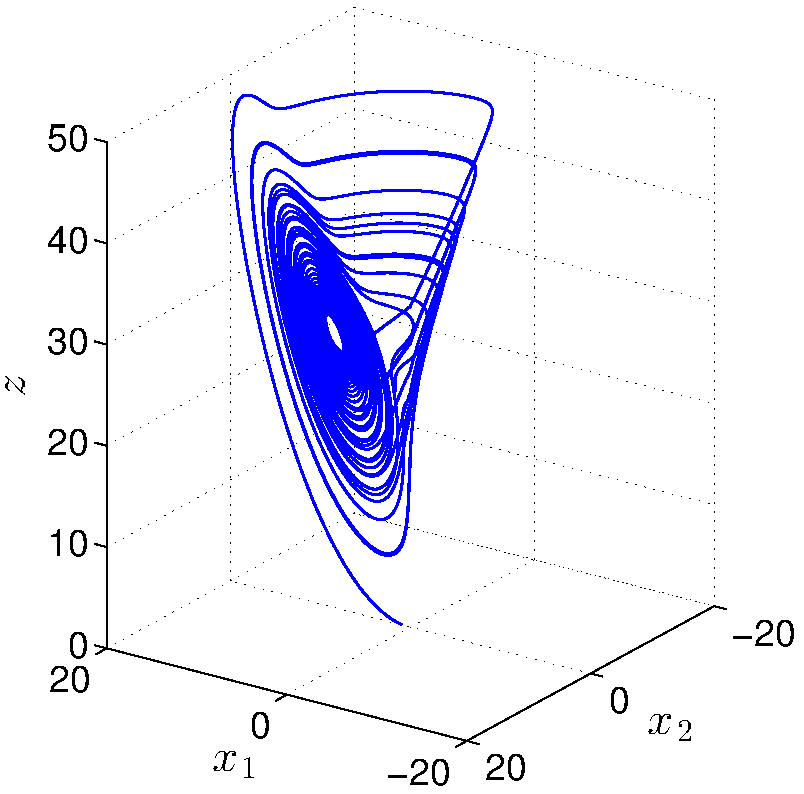
\includegraphics[width=.46\textwidth]{cmplxLorenz_nonTriv_slice}
	(b)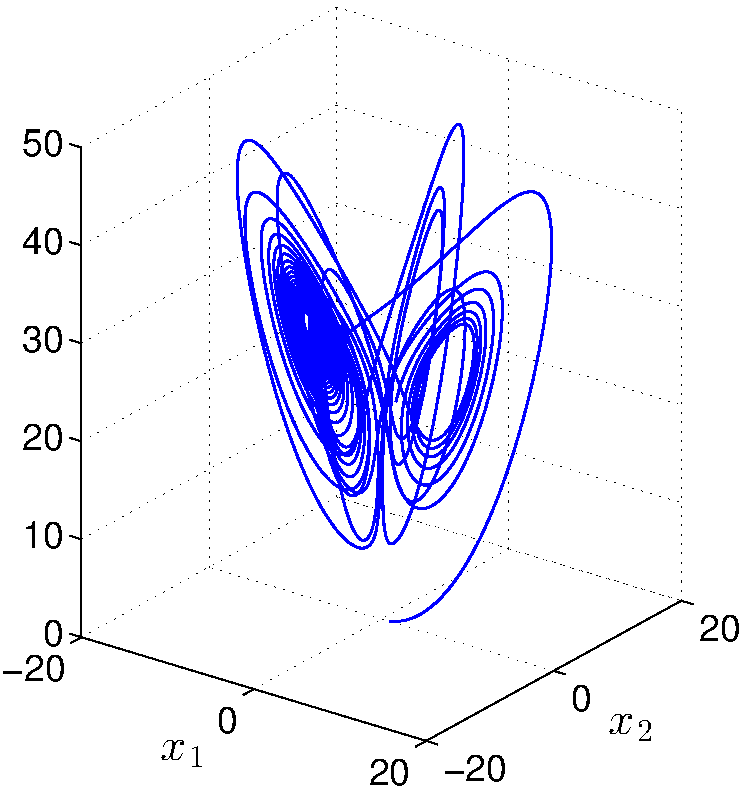
\includegraphics[width=.45\textwidth]{cmplxLorenz_movFrame}
	\caption{
A trajectory of the {\cLe} starting from the initial condition
$(1,0,1,0,0)$. (a) The non-trivial symmetry-reduced vector field
\refeq{eq:cmplxLorenz_nonTriv_slice}. (b) The co-moving frame. Note that
the co-moving frame does not reduce the symmetry.}
	\label{fig:cmplxLorenz_nonTriv_slice}
\end{figure}

Therefore we have
$$\omega_x(v(x))=\frac{-x_2 v_1+x_1 v_2}{x_1^2+x_2^2}+\frac{-y_2 v_3+y_1 v_4}{y_1^2+y_2^2},$$
and
$$\omega_x(t(x)) = 2,$$
where $v=(v_1,v_2,v_3,v_4,v_5)$ is the flow vector field for the \cLe\
and $t(x)=(-x_2,x_1,-y_2,y_1,0)$ is the symmetry group tangent at point
$x$.

Constraint \refeq{eq:const_form_02} implies
$$\dot{\theta}(x) = \frac{1}{2}\omega_x(v(x)).$$
Therefore,
\begin{equation}
u(x)=v(x)-\frac{1}{2}\left(\frac{-x_2 v_1+x_1 v_2}{x_1^2+x_2^2}+\frac{-y_2 v_3+y_1 v_4}{y_1^2+y_2^2}\right) t(x),
\label{eq:cmplxLorenz_nonTriv_slice}
\end{equation}
determines the symmetry reduced dynamics on a non-trivial `slice'.
\refFig{fig:cmplxLorenz_nonTriv_slice} shows a trajectory of $u$.
}

\MMFpost{2015-01-23}{Example:
I illustrate the differential form interpretation of 1) the
template-based slicing and 2) co-moving frame (or the method of
connections). The formulation in terms of forms shows immediately as to
why the co-moving frame does not reduce the symmetry. I use the {\cLe}
for this illustration.
	
\textit{Template-based slicing:}
In template-based slicing, one fixes a template $x'$ and take the inner
product of $t(x')=(-x_2',x_1',-y_2',y_1',0)$ with Eq. \refeq{eq:slice_vf}
to get
$$\dot{\theta}
  =\frac{\langle t(x'),v(x)\rangle}{\langle t(x'),t(x)\rangle}=\frac{ -x_2'v_1+x'_1v_2-y_2'v_3+y_1'v_4}{x_1x'_1+x_2x_2'+y_1y'_1+y_2y_2'}.$$
Comparison with \refeq{eq:const_form_02} reveals that the template-based
slicing is equivalent to taking the differential one-form to be
\beq
\omega_x = -x_2'dx^1+x_1'dx^2-y_2'dy^1+y_1'dy^2.
\ee{eq:templateForm}
Since $x'$ is fixed (constant), $\omega$ is closed, i.e. $d\omega=0$.
Therefore, the necessary condition of the theorem below is satisfied.
	
\textit{Co-moving frame:}
Now take the inner product of $t(x)$ with Eq. \refeq{eq:slice_vf} to get
$$\dot{\theta}=
\frac{\langle t(x),v(x)\rangle}{\langle t(x),t(x)\rangle}=\frac{ -x_2v_1+x_1v_2-y_2v_3+y_1v_4}{x_1^2+x_2^2+y_1^2+y_2^2}.$$
Note that $t(x)$ is not constant; it changes with the state $x$.
Comparison with \refeq{eq:const_form_02} reveals that the co-moving frame
is equivalent to choosing the differential one-form
\beq
\omega_x = -x_2dx^1+x_1dx^2-y_2dy^1+y_1dy^2.
\ee{eq:coMovFrame_form}

Its exterior derivative is
$$d\omega = 2dx^1\wedge dx^2 + 2dy^1\wedge dy^2,$$
which is non-zero, violating the necessary condition (i.e., closed-ness
of the form) for symmetry reduction.
\refFig{fig:cmplxLorenz_nonTriv_slice}(b) shows a trajectory in the
co-moving frame which exhibits a phase shift (i.e., the mysterious
geometric phase).
}

\MMFpost{2015-01-25}{Consider the differential form
\begin{equation}
\omega_x=x_2dx^1+x_1dx^2+y_2dy^1+y_1dy^2.
\label{eq:linear_form2}
\end{equation}
Note that, despite its similarity to the form \eqref{eq:coMovFrame_form}
for the co-moving frame, this form is closed, $d\omega=0$. The phase
derivative $\dot\theta$ is given by
$$\dot \theta = \frac{x_2v_1+x_1v_2+y_2v_3+y_1v_4}{x_1^2-x_2^2+y_1^2-y_2^2}$$

\refFig{fig:cmplxLorenz_nonTriv_slice_01} shows a trajectory of the
resulting symmetry-reduced vector field. It appears that the trajectory
does not reach the border, $x_1^2-x_2^2+y_1^2-y_2^2=0$, of the slice
(compare to \reffig{fig:cmplxLorenz_nonTriv_slice}(a)).
\begin{figure}[t!]
	\centering
	(a)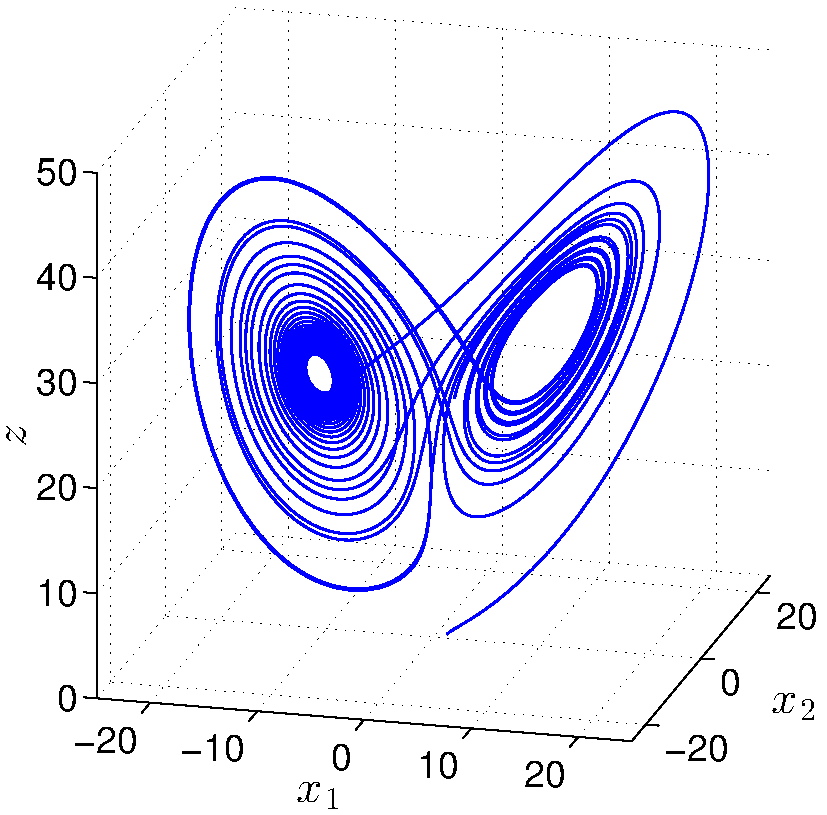
\includegraphics[width=.46\textwidth]{cmplxLorenz_nonTriv_slice_01}
	(b)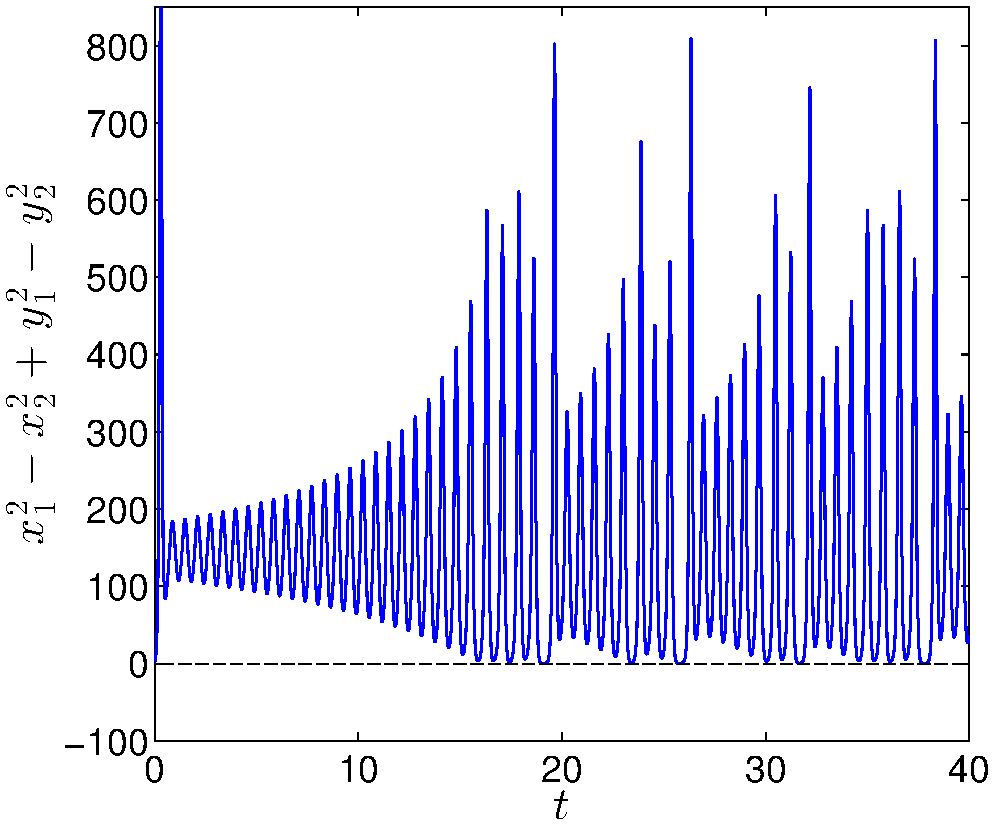
\includegraphics[width=.46\textwidth]{cmplxLorenz_sing_linearForm2}
	\caption{
(a) A trajectory of the symmetry-reduced {\cLe}  starting from the
initial condition $(1,0,1,0,0)$. For symmetry-reducing constraint
$\omega_x(u)=0$, we use $\omega_x=x_2dx^1+x_1dx^2+y_2dy^1+y_1dy^2$; see
\refeq{eq:linear_form2}. The trajectory is very similar to that of
the regular Lorenz!
(b) The evolution of the resulting denominator $x_1^2-x_2^2+y_1^2-y_2^2$
of $\dot\theta$ along the trajectory. The trajectory comes arbitrarily
close to the border (or singularities) but does not cross it.
    }
	\label{fig:cmplxLorenz_nonTriv_slice_01}
\end{figure}
}
\PCpost{2015-01-25}{
The closed form approach is great. Bunch of comments
\begin{enumerate}
  \item
I think \refeq{eq:cLeWeight1} is new (though it might turn out to be one
of many things Siminos has tried, he'll know). I do not remember us
having anything as nice for {\cLe}.
I like it, as its singularities are when either mode vanishes exactly,
hopefully that's unlikely. It would have been better if
its only singularity were on the $z$ axis,
that is an invariant subspace: the 5\dmn\ \statesp\ is not a
manifold, but an orbitfold. Perhaps that's precluded by no allowing
dependance of form $a_j=a_j(x_1,x_2,y_1,y_2)$?

\textbf{MF:} Weren't all the slices, found by Siminos, template-based? Note that \refeq{eq:cLeWeight1} is not a template-based slice: pre-factors in the differential form change along the trajectory.

  \item
Generalization to \SOn{2} and \KS\ seems straightforward.
The spatial periodicity
$u(x,\zeit)=u(x+L,\zeit)$ $\to$ Fourier space,
    \index{state space!Fourier representation}
\beq
  u(x,\zeit)=\sum_{k=-\infty}^{+\infty} \cssp_k (\zeit)\, e^{ i q_k x }
\,,
\ee{eq:ksexp}
where $\cssp_k=x_k+i\,y_k = |\cssp_k| e^{i \phi_k}$, $q_k = 2 \pi k / L$,
$L$ is the domain size, $x$ is the spatial coordinate and $\tau$ is time.
The velocity field $u(x,\zeit)$ is real, so $\cssp_k=\cssp_{-k}^\ast$,
and we can replace the sum by an $k > 0$ sum. In a truncation
a state is specified by
$2N$ real Fourier coefficients,
\beq
\ssp = (x_1, y_1, x_2, y_2, \ldots, x_N, y_N)^\mathsf{T}
\,.
\ee{repPoinExtr}
My guess is that with \refeq{eq:cLeWeight1} generalized either to
L2 norm (guessing here)
\beq
a_{k}= - k\,\frac{y_k}{x_k^2+y_k^2},\quad
b_{k}=   k\,\frac{x_k}{x_k^2+y_k^2}
\,.
\ee{eq:SO2WeightL2}
or to Sobolev $H^{-1}$ norm  (guessing here)
\beq
a_{k}=\frac{-y_k}{x_k^2+y_k^2},\quad
b_{k}=\frac{x_k}{x_k^2+y_k^2}
\,.
\ee{eq:SO2WeightH-1}
$\omega$ will be closed. Also for any other Sobolev $H^{\ell}$ norm or
indeed any other function of $k$. The $k$'s show up in
\refeq{eq:SO2WeightL2}, because I think the $\SOn{2}$ Lie algebra
generator gives you the signs in \refeq{eq:cLeWeight1}. This might be
competitive with or better than the other  symmetry reductions we
currently have.
  \item
The quickest numerical test would be on the \twomode\ equation\rf{BuBoCvSi14}.
  \item
Your second reduction \refeq{eq:linear_form2} is very simple, but seems
to be not a full symmetry reduction, but only up to a discrete \Zn{2}
subgroup of \SOn{2}. The \reqv\ around which the \cLf\ oscillates in the
full \statesp\ should reduce to an \eqv, as in
\reffig{fig:cmplxLorenz_nonTriv_slice}, not to two \eqva, as in
\reffig{fig:cmplxLorenz_nonTriv_slice_01}. The Lorenz equations indeed
have such symmetry under rotation by $\pi$, that's why we reduce the to
one-eared Van Gogh attractor.
  \item
The norms have come back from the dead...
  \item
What about Poincar\'e sections? If you do section before slice, \rpo\
torus is cut into map dynamics on a circle. Perhaps forms are not suited
to such dynamics?
  \item
Can one define slice border as condition on a differential form?
Poincar\'e section border?
  \item
You can probably find lots of computed \rpo s for \cLe\ in
\texttt{siminos} svn repository. I think also in
\\
\texttt{siminos/froehlich}. Ditto for the \twomode.
  \item
Your editor is driving svn diff batty :)

  \item \textbf{MF:} The closed-ness of the differential form is a necessary condition for the symmetry reduction. I have to find out whether it is also sufficient.

\end{enumerate}
}

\MMFpost{2015-01-26}{A comment on the closed form \refeq{eq:cLeWeight1}. If I let $a_3=a_4=a_5=0$ and keep $a_1$ and $a_2$ as they are, the reduced vector field will only have a singularity at $x_1^2+x_2^2=0$. This reduces the number of `border visits' and hence less number of sharp shifts in the trajectory. See \reffig{fig:cmplxLorenz_jumps}.
\begin{figure}[t!]
	\centering
	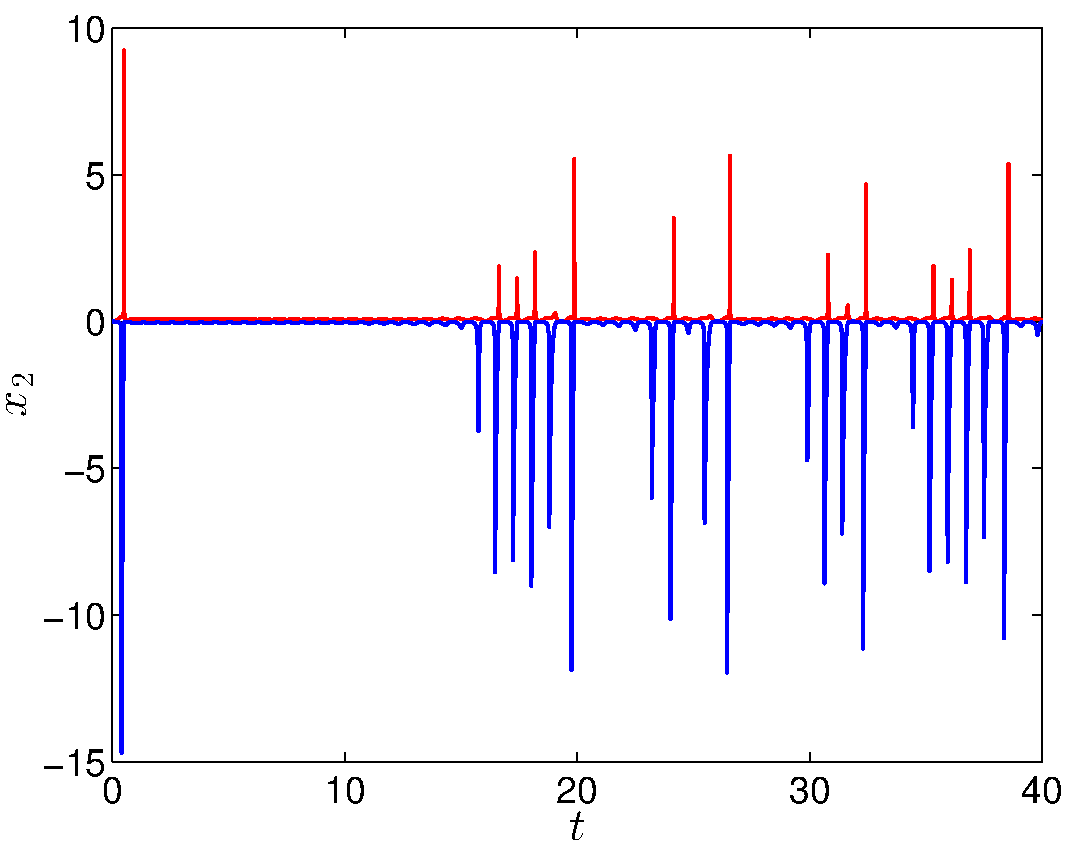
\includegraphics[width=.6\textwidth]{cmplxLorenz_jumps}
	\caption{
    Comparison between using the differential form \refeq{eq:cLeWeight1}
    (blue) and a similar differential form with $a_3=a_4=a_5=0$ (red).
    The former introduces singularities when either $x_1^2+x_2^2=0$ or
    $y_1^2+y_2^2=0$. The latter, however, only has singularities at
    $x_1^2+x_2^2=0$; hence the fewer jumps. The figure shows the
    evolution of the $x_2$ coordinate for the two reduced systems along
    the same trajectory.
	}
	\label{fig:cmplxLorenz_jumps}
\end{figure}
}

\MMFpost{2015-01-26}{It is easy to check that the differential form given by \refeq{eq:cLeWeight1} is closed. In fact, it is also exact. Define
$$f(x_1,x_2,y_1,y_2)=\tan^{-1}(x_2/x_1)+\tan^{-1}(y_2/y_1).$$
Then the differential form \refeq{eq:cLeWeight1} is given by
$$\omega_x = df(x) = \sum_{k=1}^2 \frac{\partial f}{\partial x_k}dx^k+\sum_{k=1}^2 \frac{\partial f}{\partial y_k}dy^k.$$

In general, by Poincar\'e lemma, if $U$ is a contractible open subset of $\mathbb R^n$, any \emph{smooth} closed $p$-form $\omega$ defined on $U$ is exact. That is, there exists a $(p-1)$--form $\alpha$ such that $\omega=d\alpha$.

Remark: Note that the function $f$ defined above (that is a $0$--form) is only smooth on $\mathbb R^5\backslash \{0\}$.
}

\MMFpost{2015-01-28}{Applying the symmetry reduction via differential form
$$\omega_x = \frac{-y_1}{x_1^2+y_1^2}dx^1+\frac{x_1}{x_1^2+y_1^2}dy^1,$$
to the \twomode\ equation. The constraint gives
\begin{align*}
\dot\theta(x) &= \frac{-y_1v_1(x)+x_1v_2(x)}{x_1^2+y_1^2}\\
              &= \frac{\det\begin{pmatrix}
              	x_1 & v_1\\
              	y_1 & v_2
              	\end{pmatrix}
              	}{x_1^2+y_1^2}
\end{align*}
where $v=(v_1,v_2,v_3,v_4)$ is the vector field of the \twomode\
equation, and $x=(x_1,x_2,x_3,x_4)$. See \reffig{fig:PK2} for the
results.
\begin{figure}
	\centering
	(a)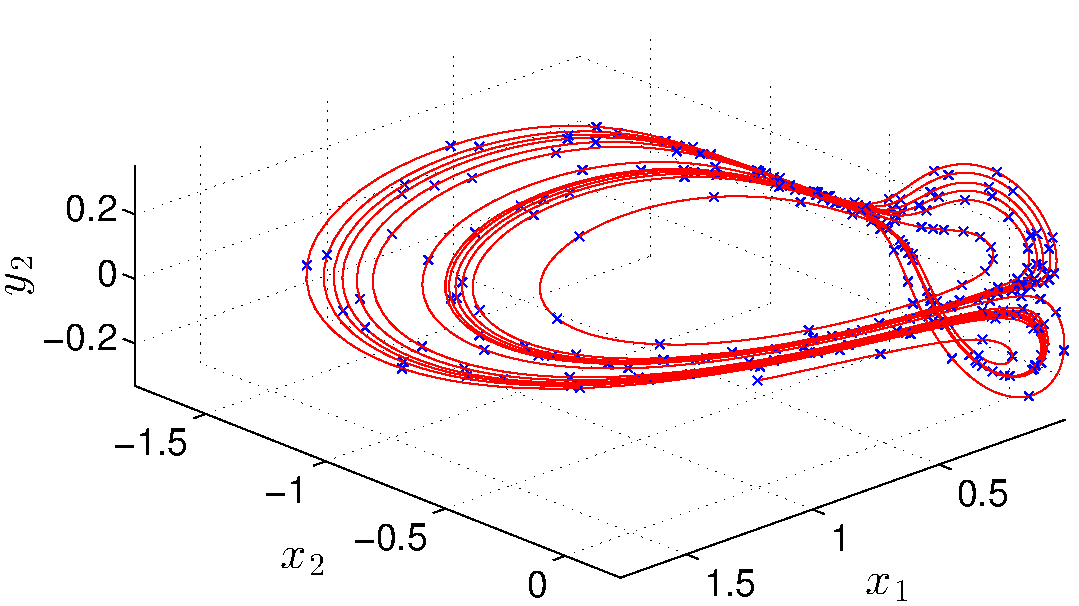
\includegraphics[width=.45\textwidth]{clForm_1stMode_PK2mode}
	(b)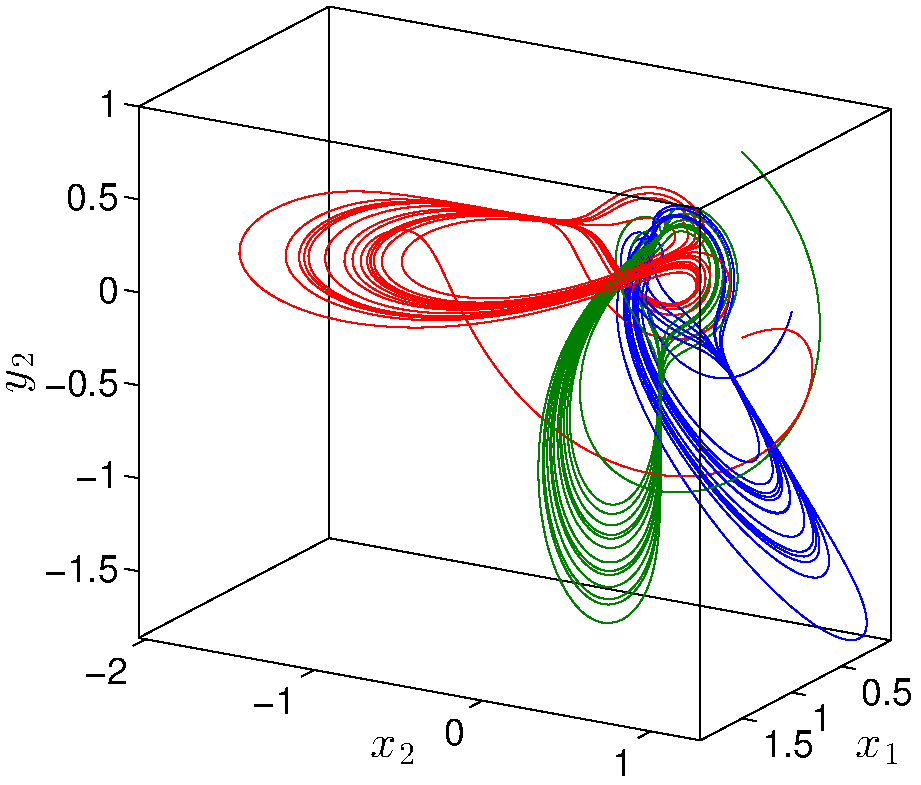
\includegraphics[width=.45\textwidth]{closedForm_PK2mode_3IC}
	\caption{
	(a) The diff. form symmetry reduction for the \twomode\ equation
        (red curve). For some reason, it coincides
        exactly with the \fFslice\ (blue crosses) [to
        be investigated...].
	(b) The initial condition for the symmetry reduction via differential form is
    	arbitrary, i.e., there is no need to bring the initial condition to the first
    	Fourier mode slice. The figure shows the symmetry-reduced trajectories starting
    	from three random initial conditions.}
	\label{fig:PK2}
\end{figure}
}

\MMFpost{2015-01-28}{I do not understand the flatness of the figures presented above:
	
I use a constraint $\omega_x(u)=0$ to uniquely determine the reduced vector field $u$.
The differential forms $\omega_x$ I use are exact, i.e., there exists a function
$f:\mathbb R^n\rightarrow\mathbb R$ such that $\omega_x = df(x)$. Therefore the
constraint $\omega_x(u)=0$ can be written as $\langle \nabla f(x),u(x)\rangle=0$. As a
result, the trajectories of $u$ are confined to the iso-surface $f(x)=f(x_0)$ where
$x_0$ is the initial condition. This hyper-surface is in general curved for a nonlinear
function $f$ (which is what I mostly use).

Why does then the attractor (for both \twomode\ and \cLe) look so flat away from the
border?
}

\MMFpost{2015-01-29}{
A formula for computing the phase change of the first Fourier mode:
	
Let $x$ be a trajectory of the reduced vector field $u=v-\dot{\theta}t$. The time evolution of the phase $\tan^{-1} (y_1/x_1)$ can be studied through its time derivative:
\begin{align*}
\frac{d}{d\tau}\tan^{-1}\frac{y_1}{x_1}&=\frac{\dot y_1 x_1-\dot x_1y_1}{x_1^2+y_1^2}\\
   & = \frac{u_2 x_1-u_1y_1}{x_1^2+y_1^2}\\
   & = \frac{(v_2-\dot{\theta}t_2) x_1-(v_1-\dot\theta t_1)y_1}{x_1^2+y_1^2}\\
   & =\frac{v_2x_1-v_1y_1}{x_1^2+y_1^2}-\dot\theta\\
   & = \frac{\alpha_x(v)}{\alpha_x(t)}-\frac{\omega_x(v)}{\omega_x(t)},
\end{align*}
where we used the fact that
$$t(x)=(-y_1,x_1,\cdots),\quad \dot\theta = \frac{\omega_x(v)}{\omega_x(t)},$$
and we define the 1-form
$$\alpha_x=-y_1dx^1+x_1dy^1.$$
We can write the above result as a 2-form:
\begin{align*}
\frac{d}{d\tau}\tan^{-1}\frac{y_1}{x_1}&=\frac{\alpha_x(v)}{\alpha_x(t)}-\frac{\omega_x(v)}{\omega_x(t)}\\
  & = \frac{\alpha_x(v)\omega_x(t)-\alpha_x(t)\omega_x(v)}{\alpha_x(t)\omega_x(t)}\\
  & = \frac{(\alpha\wedge\omega)_x(v,t)}{\alpha_x(t)\omega_x(t)}.
\end{align*}

Therefore, if we can show that the two-form $\alpha\wedge\omega$ vanishes on
$(v(x),t(x))$, for all closed forms $\omega$, then we have proved that all symmetry
reductions are equivalent to fixing the phase of the first Fourier mode!!

For instance, the differential form used in \reffig{fig:PK2}\,(a) is
$$\omega_x = \frac{-y_1}{x_1^2+y_1^2}dx^1+\frac{x_1}{x_1^2+y_1^2}dy^1.$$
It is straightforward to show that, with this choice of $\omega$,
$\alpha\wedge\omega\equiv 0$, hence the coincidence of
the \fFslice\ and differential form symmetry-reduction in that figure.
}

\MMFpost{2015-01-31}{Hill's spherical vortex is an exact solution of
the \HREF{https://www.youtube.com/watch?v=07HCb0eR9iY}{Euler}'s equations (inviscid fluid).
    \PC{2015-04-16  The thing to read is the comments on this YouTube page.
    There is an impressive number of not-too-wise persons getting STEM degrees:}
    The velocity field is given by
\begin{equation}
v(x_1,x_2,z)=\begin{pmatrix}
x_1z-2cx_2/(x_1^2+x_2^2) \\
x_2z+2cx_1/(x_1^2+x_2^2) \\
1-2(x_1^2+x_2^2)-z^2
\end{pmatrix}.
\label{eq:Hill}
\end{equation}
Note that $v$ is $SO(2)$-equivariant under rotations around the $z$ axis.
A large number of the Lagrangian trajectories, i.e., solutions of
$\dot{x}= v(x)$, with $x=(x_1,x_2,z)$, are \rpo s,
tracing invariant tori.

I hope that this simpler, easier-to-visualize model helps me understand the issue with geometric phases, etc.
}

\MMFpost{2015-01-31}{\refFig{fig:Hill} shows a trajectory of the Hill's
spherical vortex in (a) the stationary and (b) co-moving frames.

Since the group tangent is $t(x)=(-x_2,x_1,0)$, the co-moving frame vector field is given
by $u(x)=v(x)-\dot{\theta}\,t(x)$ with
$$\dot{\theta}=\frac{\langle t(x),v(x)\rangle}{|t(x)|^2}.$$

Therefore, the co-moving frame does reduce \rpo s to closed loops in three
dimensions (at least in this example). The problem with the co-moving frame only shows up
in higher dimensions. Why?
\begin{figure}
	\centering
	(a)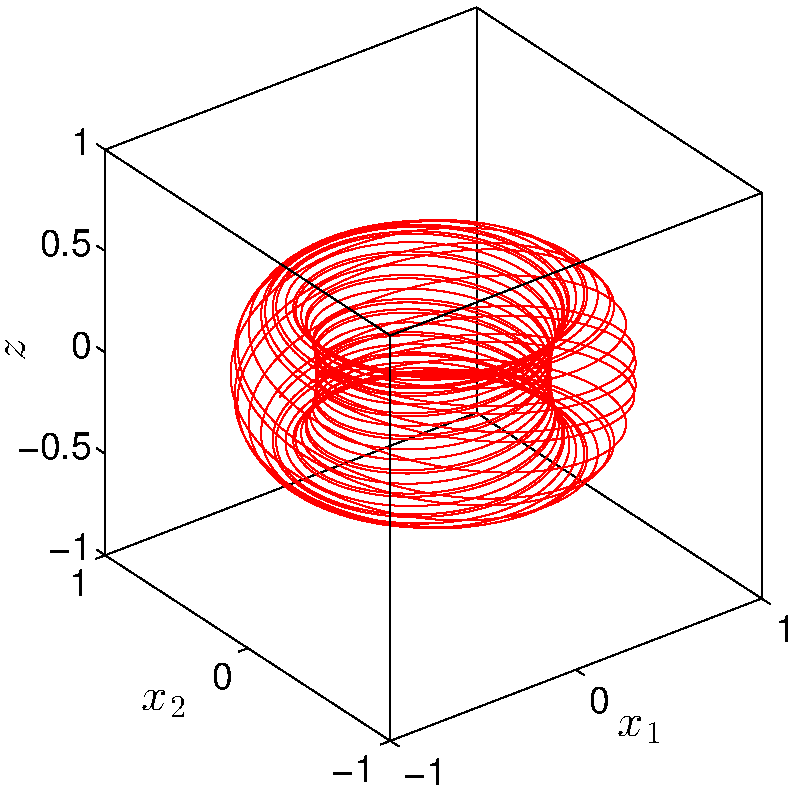
\includegraphics[width=.46\textwidth]{Hill_torus}
	(b)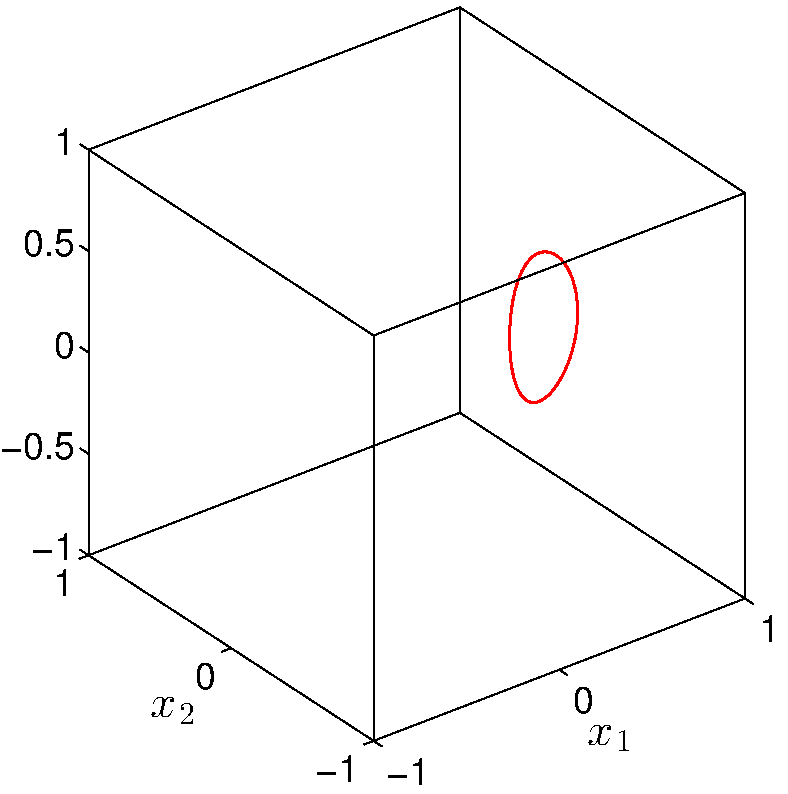
\includegraphics[width=.46\textwidth]{Hill_symRed_coMov}
	\caption{
		(a) A trajectory of the Hill's spherical vortex starting from $x=(1/2,0,0)$.
		Due to the $SO(2)$ symmetry, this is an \rpo, tracing an
		invariant torus.
		(b) The trajectory in the co-moving frame is a \po.}
	\label{fig:Hill}
\end{figure}
}

\MMFpost{2015-01-31}{
I find for Hill's vortex that the dot product of the equivariant vector field v(x) and the group tangent t(x) is conserved along \rpo s. Is this true in general for flows with \SOn{2} symmetry?

It's always true for \reqva. But I don't see why it should hold in general on \rpo s.
    }

\PCpost{2015-01-31}{
That's a big surprise for me - you know that co-moving frame depends on
choice of norm, so for \rpo s the angler to $\groupTan_{a}(\ssp)$
along general orbit $\ssp(\zeit)$ should vary. Some integrability magic?

Commit \texttt{{Hill\_torus}}.
}
\MMFpost{2015-02-01}{to Predrag: Yes, Hill's vortex is integrable...
}

\MMFpost{2015-02-02}{Why co-moving frame reduces the symmetry of Hill's vortex:

The vector field \refeq{eq:Hill} in the co-moving frame reads
\begin{equation}
u(x_1,x_2,z)=\begin{pmatrix}
x_1z \\
x_2z \\
1-2(x_1^2+x_2^2)-z^2
\end{pmatrix}.
\label{eq:Hill_coMov}
\end{equation}
We show that the trajectories of $u$ are confined to a hyperplane. Let
$x^0=(x_1^0,x_2^0,z^0)$ be an arbitrary initial conditions away from the $z$-axis. The
group tangent at this point is $t(x^0)=(-x_2^0,x_1^0,z^0)$. We show that the trajectory
$x(\tau)$ starting from $x^0$ remains in a hyperplane that includes the $z$-axis and is orthogonal to $t(x^0)$. To this end, define
$$h(\tau)=\langle x(\tau),t(x^0)\rangle = -x_2^0x_1(\tau)+x_1^0x_2(\tau).$$
Note that $h(0)=0$. Differentiate with respect to time $\tau$ to get
$$\dot h(\tau)=-x_2^0u_1(x)+x_1^0u_2(x)=z(\tau)(-x_2^0x_1(\tau)+x_1^0x_2(\tau))=z(\tau)h(\tau).$$
Rescaling time as
$$s = \int_0^\tau z(\xi)d\xi,$$
we get
$$ \frac{dh}{ds}=h(s),$$
whose solution is $h(s)=h(0)\exp(s)$. Since $h(0)=0$, we have $h\equiv 0$ for all times and therefore the trajectory $x(\tau)$ is constrained to the hyperplane defined by $\langle x,t(x^0)\rangle=0$.
}

\MMFpost{2015-02-02}{

The inner product $\langle v(\ssp),\groupTan(\ssp)\rangle$ is preserved
on \rpo s after one period:
	
Let $f^\tau:\pS\rightarrow\pS$ be the flow generated by a
vector field $v$ which is equivariant
\[
v(\LieEl \ssp)=\LieEl v(\ssp) \mbox{ for all } \LieEl \in \Group
\]
under the action of a one-parameter family of symmetry group operations
$\LieEl=\LieEl(s)$. Denote the generator of the group by
    \PC{2015-02-03 Here you are defining the group tangent field.
    You probably want to define the generator (Lie algebra, in more dimensions)
    without acting on the \statesp\ point \ssp.}
\[
\groupTan(\ssp) = \LieEl^{-1} \frac{d\LieEl }{ds}\ssp
\,.
\]
We also assume that $\pS$ is a Hilbert space with inner product
$\langle\cdot,\cdot\rangle$. The linearized group action $d\LieEl$ is
orthogonal with respect to this inner product, i.e.,
$(d\LieEl)^\top=(d\LieEl)^{-1}=d\LieEl(-s)$.
    \PC{2015-02-03 Why `linearized group action'? MF to Predrag: In the setting of the chaos book, it is assumed that $\LieEl=e^{\theta\cdot\mathbf T}$, implying that the group action $\LieEl:\ssp \mapsto \LieEl\ssp$ is linear which is the case for SO(2). This in turn means that $d\LieEl=\LieEl$. I don't think this is the case in more general settings.}

Now let $\ssp\in \pS$ be on a \rpo\ $p$, with
period $\period{p}$ and group element $\LieEl_p$ such that
$f^{\period{p}}(\ssp)=\LieEl_p \ssp$. Then
\begin{align*}
\langle v(f^{\period{}}(\ssp)),\groupTan(f^{\period{}}(\ssp))\rangle
 & = \langle v(\LieEl_p\ssp),\groupTan(\LieEl_p\ssp)\rangle\\
 &= \langle \LieEl_p v(\ssp),\LieEl_p \groupTan(\ssp)\rangle
 = \langle v(\ssp),\LieEl_p^\top \LieEl_p \groupTan(\ssp)\rangle\\
 &=\langle v(\ssp),\groupTan(\ssp)\rangle
\end{align*}
}

\MMFpost{2015-02-02}{
Symmetry reduction to curved surfaces is possible.
\refFig{fig:Hill_cubicSurf} shows a \rpo\ of Hill's spherical vortex to a
curved co-dimension-1 manifold. The manifold is the surface $x_2=x_1^3$.
\begin{figure}[t!]
		\centering
		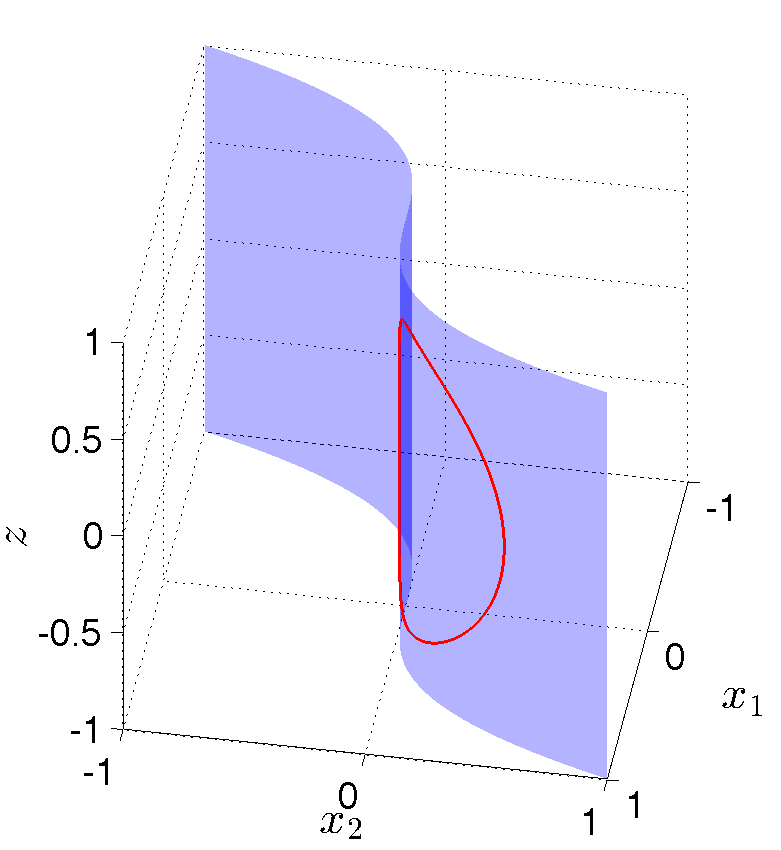
\includegraphics[width=.75\textwidth]{Hill_symRed_cubicSurf}
		\caption{
    Hill's vortex reduced to a co-dimension one manifold $\pS/\Group$ given by
    $x_2=x_1^3$ (blue surface). A \rpo\ reduces to a \po\ (red).}
		\label{fig:Hill_cubicSurf}
\end{figure}
}

\MMFpost{2015-02-02}{

Let $f^\tau:\pS\rightarrow\pS$ be the flow generated by a vector field
$v$ which is equivariant under the action of a symmetry group $\Group$,
i.e. $v(\LieEl \ssp)=\LieEl v(\ssp)$ for all $\LieEl\in\Group$. Let
$\Group$ be a one-parameter continuous symmetry group, with elements
parametrized by $s$, $\LieEl=\LieEl(s) \in \Group$.
Denote the generator of the group by $\groupTan(\ssp)$, i.e.,
    \PC{2015-02-03 Here you are defining the group tangent field.
    You probably want to define the generator (Lie algebra, in more dimensions)
    without acting on the \statesp\ point \ssp. Not sure on nomenclature.}
\[
\frac{d}{ds}\LieEl(\ssp)\Big |_{s=0}
=
\groupTan(\ssp),\quad \forall \ssp\in \pS,\; \forall \LieEl\in \Group
\,.
\]
The quotient manifold is defined through an equivalence class. The
equivalence class of a point $\ssp\in\pS$ is defined as
\[
\sspRed = \{\ssp\in\pS| \exists \LieEl\in \Group\;
   \mbox{such that}\; \LieEl(\ssp)=\sspRed\}
\,.
\]
The quotient manifold $\pS/\Group$ is the union of all such equivalence classes:
$$\pS/\Group = \bigcup_{x\in\pS}\sspRed.$$

Under certain conditions (action of $\Group$ on $\pS$ being free and
proper), the quotient manifold $\pS/\Group$ is a smooth manifold of
dimension $d-1$ where $d$ is the dimension of $\pS$.
    \PC{2015-02-02 It's probably always an orbitfold, \ie, the action
    of $\Group$ on $\pS$ is never free and proper... But it will work
    on orbitfolds.
    }

As such, $\pS/\Group$ can be embedded in $\pS$ through a co-dimension one
condition $H(\sspRed)=0$, for all $\sspRed\in \pS/\Group$. For
compatibility, the symmetry-reduced vector field $\velRed$ must preserve $H$,
\ie, the Lie derivative of $H$ with respect to $\velRed$ must vanish:
    \PC{2015-02-03 Changed ``for all $\ssp\in \pS$'' to
    ``for all $\sspRed\in \pS/\Group$''
    }
\begin{equation}
\mathcal L_{\velRed} H =0.
\label{eq:symRed_conserv}
\end{equation}

On the other hand, we know
$\velRed(\sspRed)=v(\sspRed)-\dot\theta(\sspRed) \groupTan(\sspRed)$.
The compatibility condition $\mathcal L_{\velRed} H =0$ implies
\begin{equation}
\dot\theta(\sspRed)=\frac{\mathcal L_vH}{\mathcal L_t H}\Big|_{\sspRed}.
\label{eq:compatibility}
\end{equation}


The choice of $H$ is arbitrary (it should be smooth so that the
Lie derivatives are defined).
    \PC{2015-02-03 `Arbitrary'? Cannot have $H=$(const).
    }
In \reffig{fig:Hill_cubicSurf}, I chose
$H(\ssp)=x_2-x_1^3-c$ where $c$ is determined by the initial condition
through $c=H(x_0)$.

{\bf Remarks:}
\begin{enumerate}
	\item The co-moving frame of Hill's vortex reduces the symmetry because it is equivalent
	to choosing $H(\ssp)=\tan^{-1}(x_2/x_1)$.
	
	\item I believe that the co-moving frame fails in higher dimensions
        since it does not satisfy the compatibility condition $\mathcal
        L_{\velRed} H =0$ for any scalar function $H$. I have to think
        further to make a definitive statement.
	
	\item One can readily show that the template-based slicing is a
          special case with $H(\ssp)=\langle x-x',\groupTan(x')\rangle$ where $x'$
            is the slice.
    \PC{2015-02-03 `\Slice' is not `\slicePlane': \slicePlane\ is the simplest
    example of a construction of a local chart that covers a part of the
    \slice. A \slice\ is an explicit smooth submanifold
    of the quotient manifold $\pS/\Group$, can be curvilinear \etc, but
    it is not `cross-section'. Language gets in the way quickly here...
    }

	
	\item I believe that a smart choice of $H$ may remove the border
        jumps for both  \twomode\ and \cLe.
        Ideas are needed here...
\end{enumerate}
}

\PCpost{2015-02-02}{
Does look like the one-parameter Mother of All Slices!
I recast much into ChaosBook straightjacket, with en eye on preparing
an Appendix. Good luck diffing, you $\infty$-liner!
                    }

\MMFpost{2015-02-03}{\refFig{fig:PK2_curved} shows the curved slicing for the two-mode
Porter--Knobloch using $H(x_1,y_1,x_2,y_2)=y_1-x_1^3$. \refFig{fig:PK2_flat_curved}
compares this curved slice to the first Fourier mode slicing.
		\begin{figure}[t!]
			\centering
			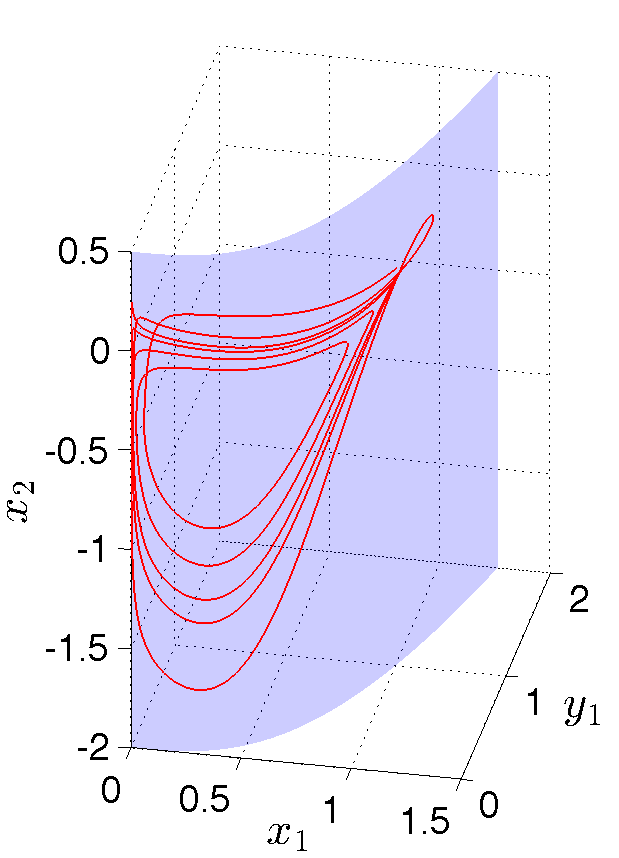
\includegraphics[width=.75\textwidth]{PK2mode_cubicSlice}
			\caption{Two-mode Porter--Knobloch with the curved slice $y_1=x_1^3$.}
			\label{fig:PK2_curved}
		\end{figure}
	\begin{figure}[t!]
		\centering
		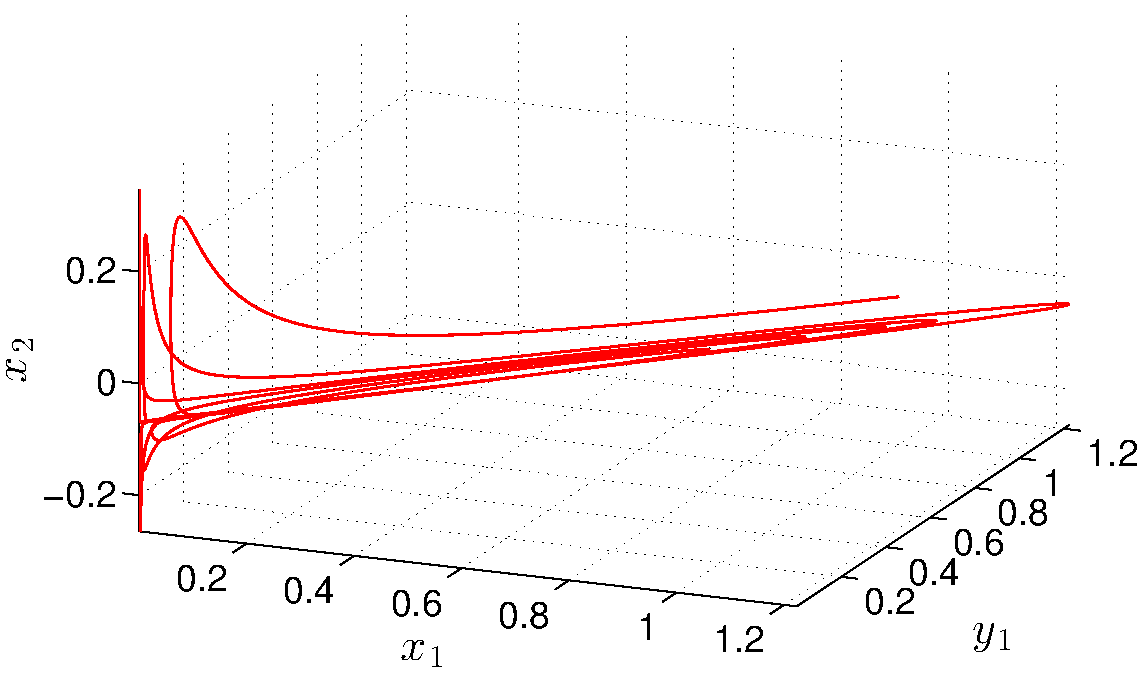
\includegraphics[width=.45\textwidth]{PK2mode_flatSlice_x1y1x2}
		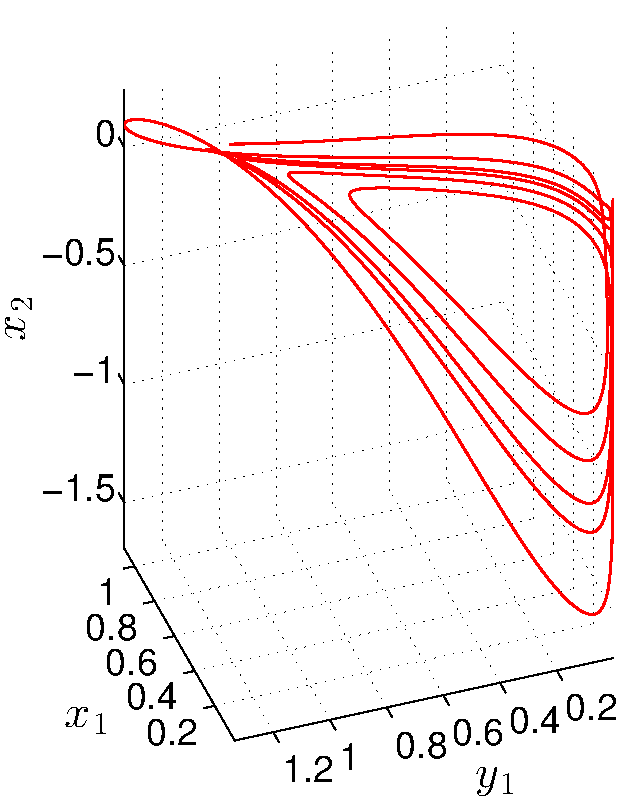
\includegraphics[width=.35\textwidth]{PK2mode_cubicSlice_x1y1x2}\\
    	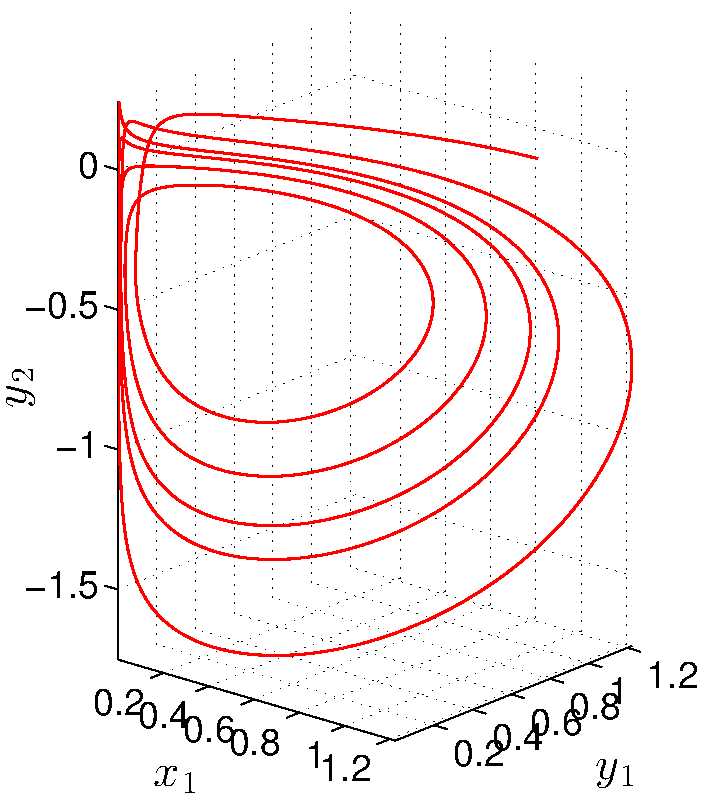
\includegraphics[width=.35\textwidth]{PK2mode_flatSlice_x1y1y2}
		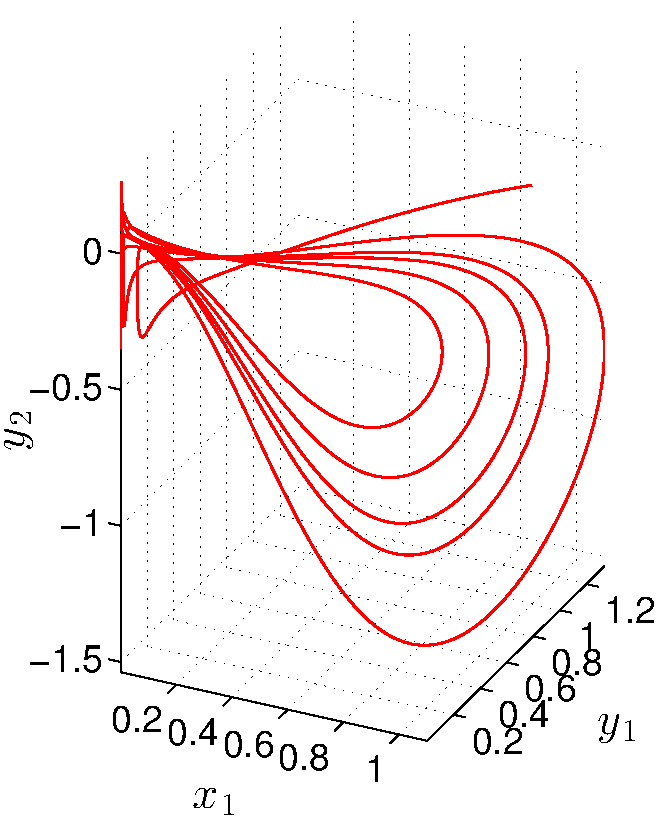
\includegraphics[width=.35\textwidth]{PK2mode_cubicSlice_x1y1y2}\\
		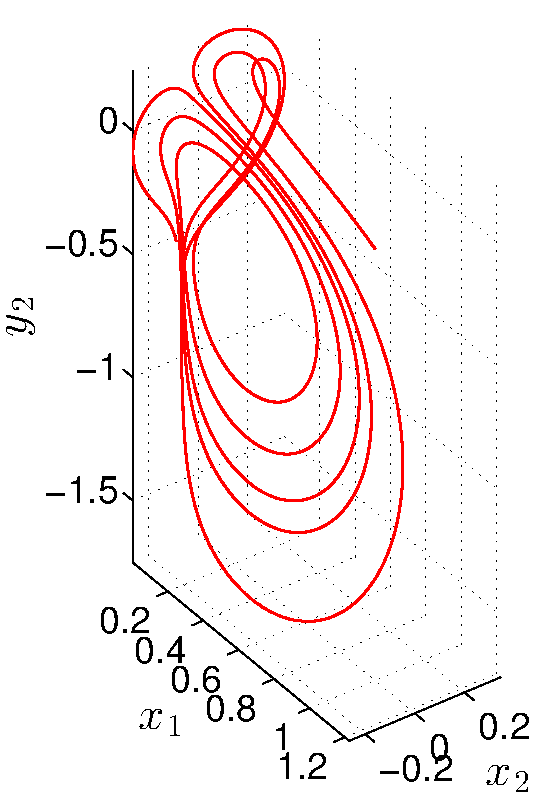
\includegraphics[width=.35\textwidth]{PK2mode_flatSlice_x1x2y2}
    	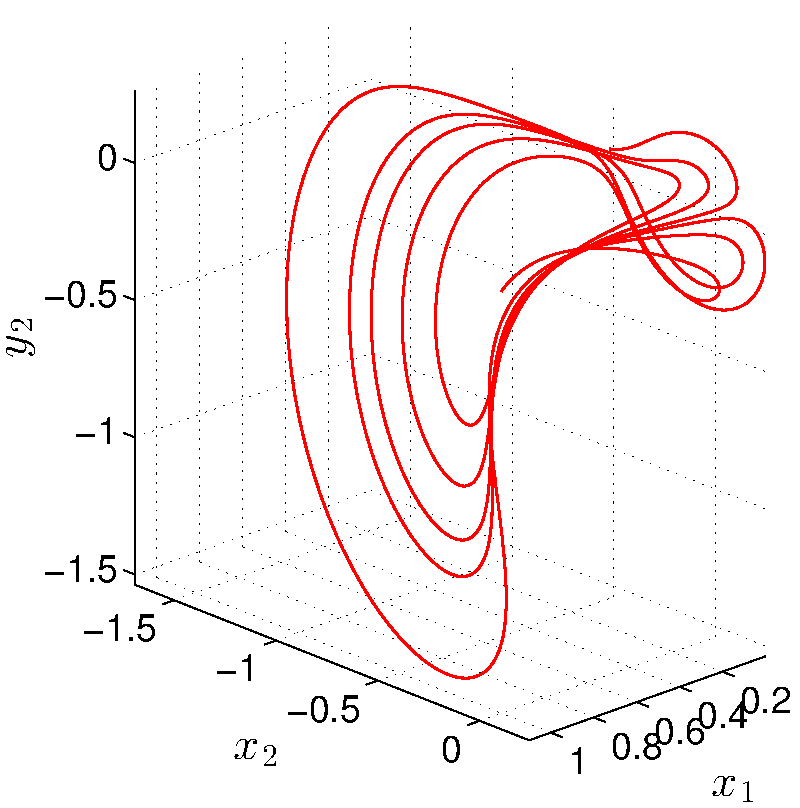
\includegraphics[width=.35\textwidth]{PK2mode_cubicSlice_x1x2y2}		
		\caption{Two-mode Porter--Knobloch with the first Fourier mode slice (left panel) and the curved slice $y_1=x_1^3$ (right panel).}
		\label{fig:PK2_flat_curved}
	\end{figure}
}
\MMFpost{2015-02-03}{Towards understanding the problem with co-moving frame (geometric
	phases):
	
So far we know that if $\velRed(\sspRed)=\vel(\sspRed) - \dot\theta(\sspRed)t(\sspRed)$ is to reduce the continuous symmetry, it must satisfy \refeq{eq:symRed_conserv} for some smooth, non-constant function $H:\pS\rightarrow \mathbb R$.

On the other hand, we know that the co-moving frame $\dot\theta(\sspRed)=\langle \vel
(\sspRed),t(\sspRed)\rangle/\langle t(\sspRed),t(\sspRed)\rangle$ does not in general reduce
the symmetry. Therefore, it suffices to show that there does not exist a function $H$ such
that $\dot\theta$ satisfies the compatibility condition \refeq{eq:compatibility}.

Proof by contradiction seems natural. Assume that there exists $H:\pS\rightarrow \mathbb R$
such that
$$\mathcal L_{\velRed}H =0, \quad \dot\theta =\frac{\langle \vel ,t\rangle}{\langle
t,t\rangle}.$$
These, together with $\velRed(\sspRed)=\vel(\sspRed) - \dot\theta(\sspRed)t(\sspRed)$, imply
$$(\mathcal L_tH)\langle \vel,t\rangle - (\mathcal L_{\vel}H)\langle t,t\rangle=0.$$


The co-moving frame already assumes the existence of an inner product on $\pS$. Therefore,
the Lie derivatives of $H$ can be written as $\mathcal L_{\vel}H=\langle \nabla
H,\vel\rangle$ and $\mathcal L_{t}H=\langle \nabla H,t\rangle$. Substituting in the equation
for $\dot{\theta}$ we get
\begin{equation}
\langle B_H(v,t),t\rangle =0,
\label{eq:compatibility_02}
\end{equation}
where
$$B_H(v,t):=\langle \nabla H,v\rangle t-\langle \nabla H,t\rangle v.$$
Properties of $B_H$:
\begin{enumerate}
	\item $B_H(v,t)\in\mbox{span}\{v,t\}$
	\item $B_H$ is skew-symmetric, i.e., $B_H(t,\vel)=-B_H(\vel,t)$.
	\item $\langle B_H(\vel,t),t\rangle =0$ (from the compatibility condition
	\refeq{eq:compatibility_02}).
	\item $\langle B_H(\vel,t),\nabla H\rangle =0$.
\end{enumerate}

{\it Remark:} Note that, $B_H$ vanishes when $v$ and $t$ are co-linear. This has
to be related to
the fact that the co-moving frame does reduce relative equilibria to equilibria.

Using the constraints listed above, I still cannot rule out the existence of a function $H$
for the co-moving frame. Any ideas?
}

\MMFpost{2015-02-04}{Perhaps, a better way to look at the compatibility condition
\refeq{eq:compatibility_02} is to rewrite it as
$$\Big\langle\langle t,t\rangle v-\langle t,v\rangle t,\nabla H\Big\rangle=0.$$
This is a linear first order PDE for $H$:
\begin{equation}
\mathcal L_a H:=a_j\frac{\partial H}{\partial x_j}=0,
\label{eq:compat_pde}
\end{equation}
with
$$a(x)=\langle t,t\rangle v-\langle t,v\rangle t.$$
The compatibility condition fails when \refeq{eq:compat_pde} does not have a solution.
This is to say, when the vector field $a$ does not admit a non-trivial first integral, the co-moving frame does not reduce the symmetry.
}

\MMFpost{2015-02-04}{Surprisingly, it seems like the literature is void of conditions
under which a given vector field does {\it not} admit non-trivial first integrals. I
could only find a conjecture by Ren\'e Thom which states \cite{ThomConj08}:

{\it ``Generically", vector
	fields on compact connected smooth manifolds without boundary can admit only trivial
	continuous first integrals}

Predrag, do you know a more useful result?

}

\PCpost{2015-02-11}{
I do not dare even think about it.
To me this question looks like on of Hilbert's open problems:)
In any case, hope the flu is not too nasty. Herbal tea and honey, doctor says.
    }

\MMFpost{2015-02-12}{I always ask the right questions! :) Yes, I feel slightly better and
dragged myself to work eventually.
}

\MMFpost{2015-02-13}{{\it Recap:} As described above, one can embed the quotient
manifold $\hat{\mathcal M}$ as the level surface of a function $H:\mathcal M\rightarrow
\mathbb R$. This implies that the symmetry-reduced vector field
$$\hat v=v-\dot \theta t,$$
leaves the surface $H=const.$ invariant. That is $H$ is a first integral of the vector
field $\hat v$ and therefore $\mathcal L_{\hat v}H=0$. This leads to the reconstruction
equation
$$\dot\theta=\frac{\mathcal L_vH}{\mathcal L_tH}.$$

{\it Problem:} The phase velocity $\dot\theta$ can in general have singularities, leading
to a potential blow up of solutions of the symmetry-reduced equation $\dot{\hat x}=\hat
v(\hat x)$. We refer to this singular set as the border. If we can show that the border
is invariant under the symmetry-reduced vector field $\hat v$, then the trajectories of
$\hat v$ stay outside of the border if they start outside it.

Here we present an example and a particular choice of the function $H$ such that the
border is indeed invariant under the symmetry-reduced vector field.

{\it Example:} Consider the complex Lorenz equation
\begin{align}
\dot x_1=-\sigma x_1+\sigma y_1,\quad \dot x_2=-\sigma x_2+\sigma y_2 & \nonumber\\
\dot y_1=(\rho_1-z)x_1-\rho_2x_2-y_1-ey_2 &\nonumber\\
\dot y_2=\rho_2x_1+(\rho_1-z)x_2+ey_1-y_2&\nonumber\\
\dot z = -\beta z+x_1y_1+x_2y_2.
\label{eq:comp_lorenz}
\end{align}

For the embedding function, we let $H(x)=x_1x_2$ and reduce the system to a level surface
$H=c$, where $c\in\mathbb R$ is a constant. We have $\mathcal L_vH = x_2v_1+x_1v_2$ and
$\mathcal L_tH = x_1^2-x_2^2$ since $t(x)=(-x_2,x_1,-y_2,y_1,0)$. Therefore,
$$\hat v(\hat x) = v(\hat x)-\frac{ \hat x_2v_1(\hat x)+\hat x_1v_2(\hat x)}{\hat
x_1^2-\hat x_2^2}t(\hat x).$$

This vector field is well-defined on the quotient manifold $\hat{\mathcal
M}=\{x\in\mathcal M: H(x)=c\}$ except on the border where $\hat x_1^2-\hat x_2^2=0$.

In order to show that this border is invariant under the flow of $\hat v$, we
define a new function $H_b(\hat x)=\hat x_1^2-\hat x_2^2$ and prove that its zero level,
surface $H_b(\hat x)=0$ ($\hat x\in\hat{\mathcal M}$), is invariant under the flow of
$\hat v$.

To this end, consider the Lie derivative of $H_b$ with respect to $\hat v$:
\begin{align}
\mathcal L_{\hat v}H_b(\hat x) &:= 2\hat x_1\dot {\hat x}_1-2\hat x_2\dot{\hat
x}_2\nonumber\\
 &=-2\sigma(\hat x_1^2-\hat x_2^2)+\sigma(\hat x_1\hat y_1-\hat x_2\hat
 y_2)+2\dot{\theta}(\hat x)H(\hat x)\nonumber\\
 &=-2\sigma H_b(\hat x)+\sigma(\hat x_1\hat y_1-\hat x_2\hat
 y_2)+2\dot{\theta}(\hat x)c,
 \label{eq:LieDer_border}
\end{align}
where for the last identity we used the definition of $H_b$ and the fact that $H(\hat
x)=c$ on $\hat{\mathcal M}$. Choose $c=0$. Then on the border, where $H_b=0$, we get
$$\mathcal L_{\hat v}H_b(\hat x)=\sigma(\hat x_1\hat y_1-\hat x_2\hat
y_2).$$
But on the border we have $H(\hat x)=\hat x_1\hat x_2=0$ and $H_b(\hat x)=\hat x_1^2-\hat
x_2^2=0$. That is the border is all the points $\{\hat x\in\hat{\mathcal M}: \hat
x_1=\hat x_2=0 \}$. Therefore, $\mathcal L_{\hat v}H_b=0$ on the border. That is
the border is invariant under the flow of $\hat v$ when the constant $c$ in
$\hat{\mathcal M}=\{x\in\mathcal M: H(x)=c\}$ is taken to be zero.

\emph{Remark:} I've seen numerically that when $c\neq 0$, my numerical integrator fails
as the trajectories do transversely cut through the border. For $c=0$, this never
happened as is suggested by the above calculation.

\emph{Caution:} Please check my calculations. I suspect that
$x_1x_2=0$ is equivalent to the first-Fourier-mode slicing (either $x_1=0$ or $x_2=0$).
We know that the border of the first-Fourier-mode slice is not invariant, right?
}

\MMFpost{2015-03-04}{Proposal to Xiong: In Riemannian geometry there is a rigorous way to define volumes and sub-volumes on a manifold $(\mathcal M,g)$ where $g$ is the Riemannian metric defined on the manifold.
	
In the absence of an intrinsic norm and since you are doing everything using $L^2$-norm, lets assume that the state space of your Kuramoto-Sivashinsky (KS) equation is equipped with the $L^2$ metric
\begin{equation}
\langle u_1, u_2\rangle = \frac{1}{L}\int_0^L u_1(x)u_2(x)dx,
\end{equation}
where $u_1$ and $u_2$ are two ``solutions" of KS (I'm omitting the dependence on time for notational simplicity) and $L$ is the length of the spatial domain.

Now let $\{\xi_1,\xi_2,\cdots\}$ be the set of \emph{unit-length} Floquet eigenvectors corresponding to the Floquet exponents $\{\lambda_1,\lambda_2,\cdots \}$, ordered such that $\Re\lambda_1>\Re \lambda_2>\cdots$.

The sub-volume $V_n$ (with respect to the $L^2$ norm) spanned by first $n$ Floquet eigenvectors $\{\xi_1,\xi_2,\cdots\xi_n\}$ is given by
\begin{equation}
V_n  = \left[\det\begin{pmatrix}
\langle \xi_1, \xi_1\rangle & \langle \xi_1, \xi_2\rangle & \cdots & \langle \xi_1, \xi_n\rangle\\
\langle \xi_2, \xi_1\rangle & \langle \xi_2, \xi_2\rangle & \cdots & \langle \xi_2, \xi_n\rangle\\
\vdots  & \vdots  & \ddots & \vdots  \\
\langle \xi_n, \xi_1\rangle & \langle \xi_n, \xi_2\rangle & \cdots & \langle \xi_n, \xi_n\rangle
\end{pmatrix}\right]^{1/2}.
\end{equation}
\textbf{Exercise:} Check that this formula gives the right value for the area of the parallelogram whose sides are the two vectors $a_1,a_2\in\mathbb R^2$. The inner product $\langle\cdot,\cdot\rangle$ is the usual Euclidean inner product instead of the $L^2$ inner product.

I would suggest the following:
\begin{enumerate}
	\item For each point $x_p$ on a (relative-) periodic orbit $p$, compute $V_n$ for $n=1,2,\cdots$. Then you can plot $V_n$ versus $n$.
	\item Repeat this for all points along $p$. Then plot the ensemble average $\langle V_n\rangle_{x_p}$ versus $n$ where the ensemble average is taken over all points $x_p$ belonging to $p$.
	\item Next, repeat this for all (relative-) periodic orbits $p$.
\end{enumerate}

This is a statistical approach and I'm not sure what the outcome would be. But if there is any merit to the proposal that unimportant modes are ``orthogonal" to the inertial manifold and important modes are ``entangled", I would expect the following: For small $n$, $\langle V_n\rangle$ has relatively small values, but as $n$ increases you should see a sharp jump in your plot at some distinguished dimension $n=n_c$.
}

\item[Xiong 2015-3-5]
In previous figure, I treated the determinant as the volume wrongly, but in
\reffig{fig:volFloquet}, I took the square root of the determinant
to get the volume. I think \reffig{fig:volFloquet} makes sense because
when a perpendicular vector is added to the subspace, the volume does not
change, just like you add a vertical axis to a rectangle in x-y plane
to form a cube, the
volume is still the area of this square, if the added vector is normalized.
However, if the added vector is not perpendicular to the present set,
then volume will shrink.
  \begin{figure}
    \centering
    (a)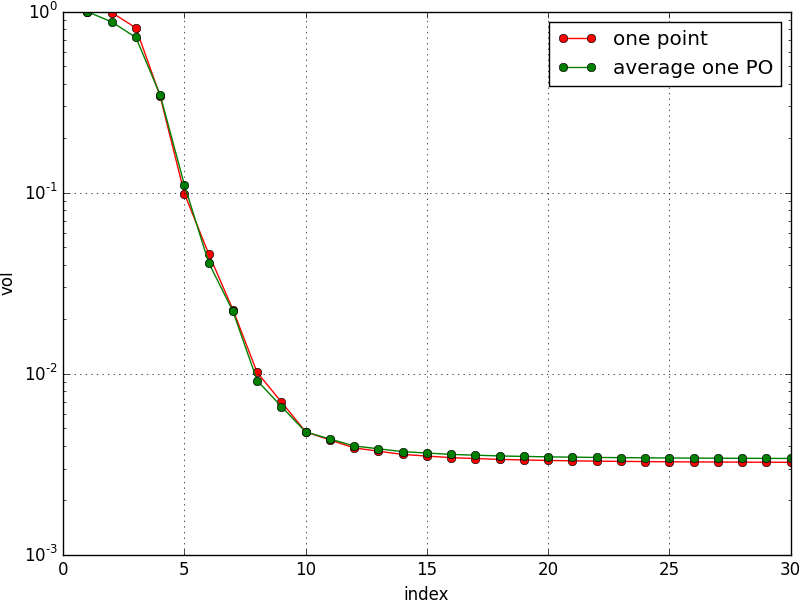
\includegraphics[width=0.45\textwidth]{vol}
    (b)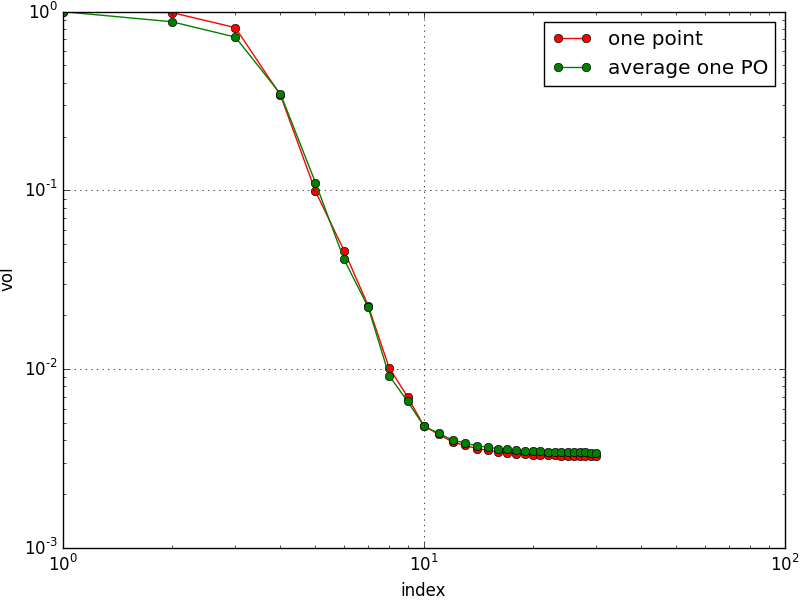
\includegraphics[width=0.45\textwidth]{vol2}
    \caption{volume versus the number of Flouqet vectors. (a) and
      (b) are the same, but (b)'s has x-log scale.
    }
    \label{fig:volFloquet}
  \end{figure}

\MMFpost{2015-03-05}{Xiong, you are absolutely right. As you said, it makes sense for the
sub-volume $V_n$ to decrease as $n$ increases. }

\MMFpost{2015-03-05}{Xiong, your sub-volume figure is promising. In
\reffig{fig:subVol_30}, I plot the same thing as you but I take $n$ randomly chosen
vectors in $\mathbb R^{30}$ where $n$ increases from $1$ to $30$. For each $n$, I compute
the sub-volume $V_n$. Note that the volume of $n$ randomly chosen vectors shrinks
(super-) exponentially while your plot has a plateaus around $n>15$.
  \begin{figure}
  	\centering
  	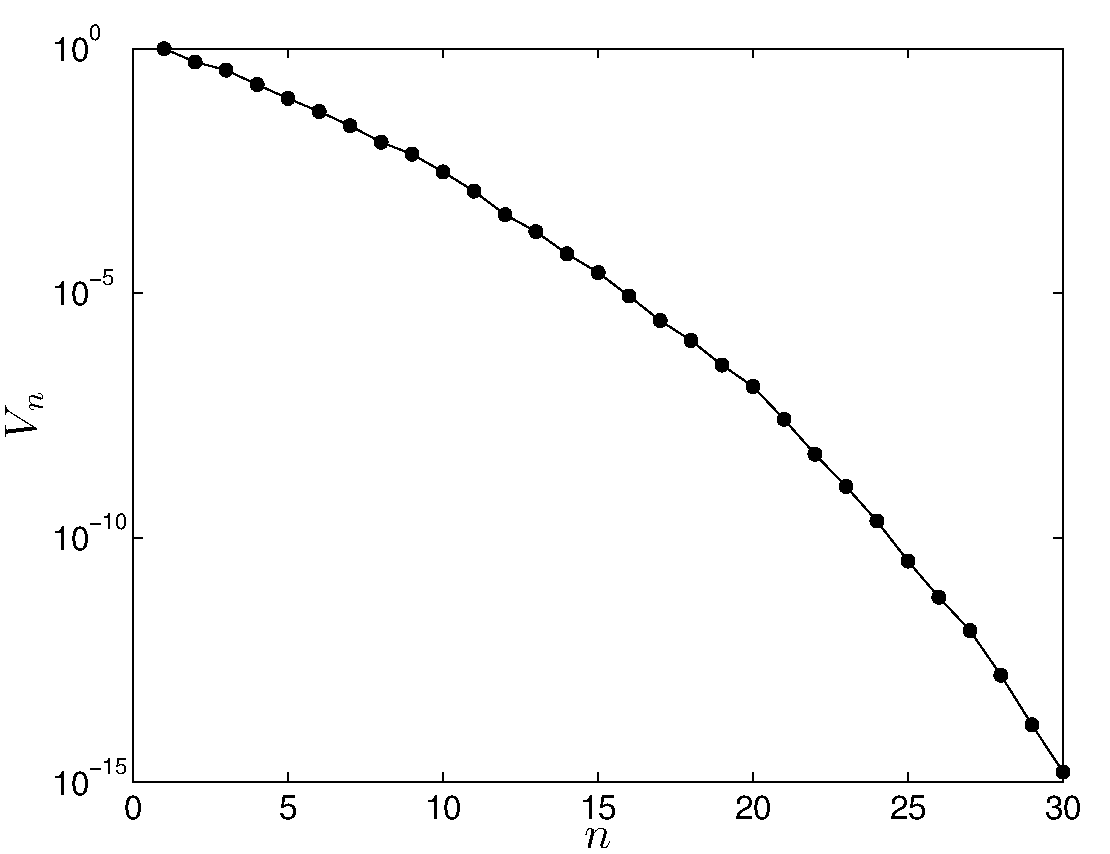
\includegraphics[width=0.75\textwidth]{subVol_30}
  	\caption{The sub-volume $V_n$ formed by $n$ randomly chosen vectors in $\mathbb
  	R^{30}$.
  	}
  	\label{fig:subVol_30}
  \end{figure}
	}
\end{description}
